\documentclass{llncs}
\usepackage[T1]{fontenc}
\usepackage[utf8]{inputenc}

%% \usepackage{fontspec}
%% \newfontfamily{\tam}[Script=Tamil]{Lohit Tamil}
%% \defaultfontfeatures{Scale=MatchLowercase}

\usepackage{eurosym}
\usepackage{hyperref}		% clickable references
\usepackage{amsmath,amssymb}	% math structures and symbols
\usepackage{graphicx}		% including of graphics files in various formats
\usepackage{amsfonts}
\usepackage{dialogue}
\usepackage{placeins}
\usepackage{tikz}
\usetikzlibrary{positioning,backgrounds,fit,arrows,shapes,shadows}
\usetikzlibrary{shapes.multipart}
\usepackage{wrapfig}
\usepackage{enumitem}
\usepackage{framed}

\hypersetup{hidelinks}

\usepackage[xspace,mla]{ellipsis}

\definecolor{myyellow}{RGB}{242,226,149}
\definecolor{mygreen}{RGB}{144,238,144}
\definecolor{mypink}{RGB}{255,182,193}
\definecolor{myorange}{RGB}{255,165,0}
\definecolor{myblue}{RGB}{0,204,204}

\usepackage{xparse}
\NewDocumentCommand\StickyNote{O{4cm}mmO{4cm}}{%
\begin{tikzpicture}
\node[
drop shadow={
  shadow xshift=2pt,
  shadow yshift=-4pt
},
inner xsep=7pt,
fill=#2,
xslant=-0.05,
yslant=0.05,
inner ysep=10pt
] {\parbox[t][#1][c]{#4}{#3}};
\end{tikzpicture}%
}

\urldef{\mailsa}\path|{j.corneli,s.colton}@gold.ac.uk|
\urldef{\mailsb}\path|a.pease@dundee.co.uk|

\newcommand{\keywords}[1]{\par\addvspace\baselineskip
\noindent\keywordname\enspace\ignorespaces#1}

\begin{document}

% TITLE INFORMATION
\title{Modelling serendipity in a computational context}
\author{Joseph Corneli\inst{1}, Alison Pease\inst{2}, Simon Colton\inst{1},\\ Anna Jordanous\inst{3}, Christian Guckelsberger\inst{1}}
\date{\today}
\institute{Department of Computing, Goldsmiths College, University of London\\
%% \mailsa\\
%% \mailsb\\
\url{http://ccg.doc.gold.ac.uk/}
\and
School of Computing, University of Dundee
\and
School of Computing, University of Kent}

\maketitle

\begin{abstract} 
Drawing on well-known examples of serendipity in scientific discovery,
we develop a set of criteria that can be applied to model and evaluate
serendipity in computational settings.  We use design patterns, and
the growth of a pattern language, as a way to describe the processes
of discovery and invention that comprise serendipitous encounters.  We
show how several earlier patterns of serendipity can be applied in a
Writers Workshop for computational systems, and include related
recommendations for practitioners.  \\[.5cm]
%
\keywords{serendipity,
design patterns,
intelligent machinery,
Writers Workshops}
\end{abstract}

\section{Introduction}

Materials, like gold, and processes, like metalurgy, have no value
without a context of application: decoration, trade, circuitry, and so
on.  In practice, we are likely to attribute \emph{value} to materials that
are useful, and \emph{creativity} to a person who puts materials to use in a
novel way.
%
Many instances of \emph{serendipity} centre on reevaluation.  For
example, a non-sticky ``superglue'' that no one was quite sure how to
use turned out to be just the right ingredient for 3M's
Post-it\texttrademark\ notes.
%
Serendipity is related, firstly, to deviations from familiar patterns,
and secondly, to new insight.
%
When we consider the practical uses for weak glue, the possibility
that a life-saving antibiotic might be found growing on contaminated
petri dishes, and or the idea that cockle-burs could be anything but
annoying, we encounter radical changes in the evaluation of what's
interesting.  In the \emph{d\'enouement}, what was initially
unexpected is found to be both explicable and useful.

Van Andel \cite{van1994anatomy} -- echoing Poincar\'e's
\cite{poincare1910creation} (negative) reflections on the potential
for a purely computational approach to mathematics -- claimed that:
\begin{quote}
``\emph{Like all intuitive operating, pure serendipity is not amenable
    to generation by a computer.  The very moment I can plan or
    programme `serendipity' it cannot be called serendipity
    anymore}.'' \cite{van1994anatomy}
\end{quote}
We believe that serendipity is not so mystical as such statements
might imply, and in Sections \ref{sec:patterns-of-serendipity} and
\ref{sec:computational-serendipity} we will show how it is possible to
reinterpret van Andel's ``patterns of serendipity'' in computational
settings.  

The real problem with computers is not that they only do what they're
told, but that the act of programming forces us to confront the
emergence of the new \cite{mead1932philosophy}.
%
Minsky \cite{minsky1967programming} suggests that in practice,
programmers write programs ``for the individuals of little societies''
precisely because we cannot envision in advance all of the details of
program interactions.
%
Indeterminacy forms an important part of any proposal for
``intelligent machines'', after Turing:
\begin{quote}
``\emph{They will make mistakes at times, and at times they may make
    new and very interesting statements, and on the whole the output
    of them will be worth attention to the same sort of extent as the
    output of a human mind}.''  \cite{turing-intelligent}
\end{quote}

Serendipity has played a role in the large-scale history of the
computing field \cite{de2013turing} and in artistic applications of
computer technology \cite{reichardt1969cybernetic}.  We aim to clarify
the role it has to play in the future development of computational
creativity.

Whereas van Andel speaks of ``patterns of serendipity'' in a
relatively informal way, this paper will rely on the somewhat more
formal theory of \emph{design patterns} \cite{alexander1999origins},
to which it makes several additions and alterations.  This theory is
by no means limited to computing, and indeed, has its origins in
architecture and urban planning.  Our approach to ``designing for
serendipity'' \cite{andre2009discovery} centres on the use of design
patterns to capture the dynamic aspects of serendipitous situations.

The typical use of design patterns, since they were introduced by
Christopher Alexander
\cite{alexander1979timeless,alexander1977pattern}, is to prescribe as
well as to describe.  Design patterns provide models \emph{for} as
well as models \emph{of} (cf. \cite[p. 93]{geertz1973interpretation}).
Thus, when Alexander describes the pattern \emph{A place to wait}, he
is telling readers that it is a good idea to consider building such
places when designing living spaces.  In connection with our
understanding of serendipity as closely associated with deviations
from familiar patterns, the central concern in this paper is the way
in which \emph{new} patterns are formed.

For example, when Poincar\'e \cite{poincare1910creation} describes his
discovery of the existence of Fuchsian functions, he includes the
detail: ``contrary to my habit I took black coffee, I could not
sleep.''  This is much more interesting as part of a story about an
exceptional case of productive insomnia than it is as the broad
characterisation of a typical nightly sleep schedule.  It might best
be described as a part of a ``situational pattern,'' with a title like
\emph{Change of pace}, rather than a ``behaviour pattern''; indeed, at
the level of behaviour, a \emph{Change of pace} is the exception to a
pattern!  Nevertheless, along with Poincar\'e, we can recognize a
pattern at another level.

The key idea in this paper is to computationally model situations
where emergence of this particular sort can happen.
%
It will take some work to get there, however.  Section
\ref{sec:literature-review} develops 13 key criteria for the
evaluation of serendipity based on a review of several well-known
examples of serendipitous discoveries from human history.  Section
\ref{sec:foundations} describes a working testbed for exploring
serendipitous computational discovery.  In Section
\ref{sec:patterns-of-serendipity}, we apply our 13 criteria to analyse
several narrative ``patterns of serendipity'' collected by van Andel
\cite{van1994anatomy}.  Section \ref{sec:patterns-of-serendipity} is
the theoretical core of the paper; here we give our interpretation of
the design pattern methodology.  In Section
\ref{sec:computational-serendipity}, we focus on serendipity in a
computational context, condensing our criteria into an operational
definition, making our treatment of design patterns more concrete, and
proposing an experimental setup that we think will exhibit many of the
relevant features.  In Section \ref{sec:related}, we examine related
work, and in Section \ref{sec:recommendations}, we advance our
recommendations for researchers working on computational creativity
(and serendipity).

\section{Literature review} \label{sec:literature-review}

In this section, we give a short overview covering the etymology of
the term ``serendipity'' and trace its development in order to pin
down the key commonalities from many definitions and instances.  In
particular, we point out key conditions of serendipity, their
components and general characteristics, including environmental
factors.  The structure of this section follows and updates an earlier
survey from Pease et al.~\cite{pease2013discussion}.

\subsection{Etymology and selected definitions} \label{sec:overview-serendipity}
The English term ``serendipity'' derives from the 1302 long poem ``Eight Paradises'', written in Persian by the Sufi poet Am\={\i}r Khusrow in Uttar Pradesh.\footnote{\url{http://en.wikipedia.org/wiki/Hasht-Bihisht}}  In the English-speaking world, its first chapter became known as ``The Three Princes of Serendip'', where ``Serendip'' represents the Old Tamil-Malayalam word for Sri Lanka (%{\tam சேரன்தீவு},
\emph{Cerantivu}), ``island of the Ceran kings.''

The term ``serendipity'' is first found in a 1557 letter by Horace Walpole to Horace Mann:
\begin{quote}
\emph{``This discovery is almost of that kind which I call serendipity, a very expressive
word} \ldots \emph{You will understand it better by the derivation than by the
definition. I once read a silly fairy tale, called The Three Princes of Serendip:
as their Highness travelled, they were always making discoveries, by accidents
\& sagacity, of things which they were not in quest of}[.]''~\cite[p. 633]{van1994anatomy}
\end{quote}
The term became more widely known in the 1940s through studies of serendipity as a factor in scientific discovery, surveyed by Robert Merton and Elinor Barben \cite{merton} in their 1957 analyis ``The Travels and Adventures of Serendipity, A Study in Historical Semantics and the Sociology of Sciences''.  Merton and Barben define the term as follows:
\begin{quote}
\emph{``The serendipity pattern refers to the fairly common experience of observing
an unanticipated, anomalous and strategic datum which becomes the occasion
for developing a new theory or for extending an existing theory.''} \cite[p. 635]{van1994anatomy}
\end{quote}
In 1986, Philippe Qu\'eau described serendipity as ``the art of
finding what we are not looking for by looking for what we are not
finding'' \cite{eloge-de-la-simulation}, as quoted in
\cite[p. 121]{Campos2002}.  Pek van Andel describes it simply as ``the
art of making an unsought finding'' \cite[p. 631]{van1994anatomy}.

Roberts \cite[pp. 246--249]{roberts} records 30 entries for the term ``serendipity'' from English language dictionaries dating from 1909 to 1989.  
%
Classic definitions require the investigator not to be aware of the problem they serendipitously solve, but this criterion has largely dropped from dictionary definitions. Only 5 of Roberts' collected definitions explicitly say ``not sought for.''  Roberts characterises ``sought findings'' in which an accident leads to a discovery with the term \emph{pseudoserendipity} \cite{chumaceiro1995serendipity}.
%
While Walpole initially described serendipity as an event (a discovery), it has since been reconceptualised as a psychological attribute, a matter of sagacity on the part of the discoverer: a ``gift'' or ``faculty'' more than a ``state of mind.''  Only one of the collected definitions, from 1952, defined it solely as an event, while five define it as both event and attribute.

However, there are numerous examples that exhibit features of
serendipity which develop on a social scale rather than an individual
scale.  For instance, between Spencer Silver's creation of high-tack,
low-adhesion glue in 1968, the invention of a sticky bookmark in 1973,
and the eventual launch of the distinctive canary yellow re-stickable
notes in 1980, there were many opportunities for
Post-its\texttrademark\ \emph{not} to have come to be
\cite{tce-postits}. Accordingly, Merton and Barber argue that the
psychological perspective needs to be integrated with a
\emph{sociological} one.\footnote{ ``For if chance favours prepared
  minds, it particularly favours those at work in microenvironments
  that make for unanticipated sociocognitive interactions between
  those prepared minds. These may be described as serendipitous
  sociocognitive microenvironments'' \cite[p. 259--260]{merton}.}
Large-scale scientific and technical projects generally rely on the
``convergence of interests of several key actors''
\cite{companions-in-geography}, along with other supporting cultural
factors.  Umberto Eco \cite{eco2013serendipities} focuses on the
historical role of serendipitous mistakes and falsehoods in the
production of knowledge.

It is important to note that serendipity is usually discussed within
the context of \emph{discovery}, rather than \emph{creativity},
although in typical parlance these terms are closely related
\cite{jordanous12jims}.  Henri Bergson's distinction will be useful in
what follows:
\begin{quote}
``\emph{Discovery, or uncovering, has to do with what already exists,
    actually or virtually; it was therefore certain to happen sooner
    or later.  Invention gives being to what did not exist; it might
    never have happened.}''~\cite{bergson2010creative}
\end{quote}
Serendipity, as we understand the term, would seem to require features
of both; that is, the discovery of something unexpected and the
invention of an application for the same.  We must complement analysis
with synthesis \cite{delanda1993virtual}.  The balance between these
two features will differ from case to case.  In the following section,
we will elaborate on the characteristics of serendipity with
particular reference to classic examples.

\subsection{Characteristics of serendipity}\label{sec:characteristics}

Here we will describe our key condition for serendipity, the presence
of a Focus Shift, together with four key components that implement
this (Prepared Mind, Serendipity Trigger, Bridge, Result), four
dimensions that are generally present to some degree in instances of
serendipitous discovery or invention (Chance, Curiosity, Sagacity,
Value) and four supporting environmental factors that, if not strictly
required, are at least conducive to serendipity (Dynamic world,
Multiple contexts, Multiple tasks, Multiple influences). We shall relate these descriptions to some of the most famous examples of serendipity.
With the characteristics in mind it is not hard to spot further examples.
%% with similar characteristics: e.g. the invention of dry cleaning by
%% a professional dye-maker after his maid spilled kerosene on the
%% tablecloth, or the discovery of a marketable use for sildenafil
%% citrate (better known as {\em Viagra}\texttrademark) which had been
%% trialled as a heart medicine.

\begin{itemize}
\item The 17\textsuperscript{th} Century discovery that \emph{quinine} extracted from
  the bark of South American cinchona trees could be used to treat and
  prevent malaria -- building on a much earlier indigenous Quechua
  discovery that the extract stops shivering.
\item Fleming's discovery of {\em penicillin}.\footnote{Merton and
  Barber \cite{merton} state that the description of this discovery
  was the first time that the word \emph{serendipity} was used without
  inverted commas or accompanying definition.}
\item de Mestral's invention of {\em Velcro}\texttrademark\ following
  the model presented by cockle-burs that stuck to his jacket while
  out walking \cite[pp 220-222]{roberts}.
\item Arthur Fry's invention of sticky bookmarks (the prototype for
  {\em Post-it}\texttrademark\ notes), using a weak glue developed by
  his colleague, Spencer Silver \cite[p. 224]{roberts}.
\item Penzias and Wilson's discovery of the {\em echoes of the Big
  Bang} \cite{singh2004big}.
\item Kekul\'e's dream-inspired discovery of the {\em structure of the
  benzine ring} \cite[p. 21]{benfey}, cf. \cite[p. 77]{roberts}.
\item Charles Goodyear's invention of {\em vulcanised rubber}
  \cite{goodyear1855gum}.
\item The {\em Rosetta Stone} was found by a soldier who was
  demolishing a wall in order to clear ground for what was to be Fort
  St. Julien \cite[pp. 109 - 111]{roberts}.
\end{itemize}

\subsubsection*{Key condition for serendipity}

\paragraph{Focus shift.}
The most extreme cases show focus establishing itself as if from
nowhere: de Mestral was walking through the Alps when he encountered
the ``seeds'' of his discovery.
\begin{quote}
``\emph{After removing several of the burdock burrs (seeds) that kept sticking to his clothes and his dog's fur, he became curious as to how it worked. He examined them under a microscope, and noted hundreds of `hooks' that caught on anything with a loop, such as clothing, animal fur, or hair. He saw the possibility of binding two materials reversibly in a simple fashion, if he could figure out how to duplicate the hooks and loops.}''~\cite{wiki:velcro}
\end{quote}
In some cases, the focus shift takes place within a social context:
Arthur Fry and Spencer Silver had different ideas about what could be
done with weak glue.
%
In all of the discoveries listed above, there was a radical change in
the discoverer's evaluation of what is interesting.  We can think of
this as a reclassification of ``noise'' to ``signal.''

\subsubsection*{Components of serendipity}

\paragraph{Prepared Mind.}

Kekul\'e's ``prepared mind'' included his focus on the problem of
finding the structure of the benzine molecule and his knowledge and
skill as a scientist.  Fleming's ``prepared mind'' included his focus
on carrying out experiments to investigate influenza as well as his
previous experience that foreign substances in petri dishes can kill
bacteria.  He was concerned above all with the question ``Is there a
substance which is harmful to harmful bacteria but harmless to human
tissue?''  \cite[p. 161]{roberts}.  The social analogues are clear:
for example, 3M not only had a talented staff, but ran internal
technical forums where staff members could exchange ideas.
 
\paragraph{Serendipity Trigger.}

The trigger does not directly cause the outcome, but rather, inspires
thought.  Indeed, the trigger may bear very little resemblance to the
eventual result.  On its own, the trigger would not typically be seen
as an important discovery.  Examples include a dream, a petri dish
with a clear area, and cockle-burs attached to a jacket.  In a social
context, the trigger may have several parallel or sequential
components, and may rely on the circumstantial alignment of interest
between different parties.  For example, it was long known that
cinchona bark stops shivering; in particular, it stops shivering in
malaria patients, as was observed when malarial Europeans arrived for
the first time in Peru.  That it additionally can cure and can even
prevent malaria was subsequently revealed.

\paragraph{Bridge.}

The bridge is what affords movement from the trigger to the result.
These include reasoning techniques, such as abductive inference (what
might cause a clear patch in a petri dish?); analogical reasoning (de
Mestral constructed a target domain from the source domain of burs
hooked onto fabric); and conceptual blending (Kekul\'e blended his
knowledge of molecule structure with his vision of a snake biting its
tail).  The bridge may also rely on new social arrangements, such as
the formation of cross-cultural research networks
\cite{companions-in-geography}.

\paragraph{Result.}

This is the outcome itself. This may be a new product, artefact,
process, hypothesis, a new use for a material substance, and so on.
The outcome may contribute evidence in support of a known hypothesis,
or a solution to a known problem.  Alternatively, the result may
itself be a {\em new} hypothesis or problem.  The result may be a
``pseudoserendipitous'' in the sense that it was {\em sought}, while
nevertheless arising from an unknown, unlikely, coincidental or
unexpected source.  More classically, it is an \emph{unsought}
finding, such as the discovery of the Rosetta stone.


\subsubsection*{Dimensions of serendipity}


\paragraph{Chance.}

The {\em serendipity trigger} tends to be unlikely, unexpected,
unsought, accidental, random, or coincidental.  The trigger has
features that arise independently of the result, and even
independently of any search for a result.  The relevant features may
be ``hidden in plain view,'' and chance may apply to the conditions
that eventuate in their discovery, as when malarial Europeans chanced
upon a remedy found only in South America.  Fleming \cite{fleming}
noted: ``There are thousands of different moulds'' -- and ``that
chance put the mould in the right spot at the right time was like
winning the Irish sweep.''

\paragraph{Curiosity.}

The capacity for keeping an \emph{open mind}, and the corresponding
ability to take advantage of the unpredictable, is necessary for a
focus shift to take place.  Many of the investigators described above
went beyond simply keeping an open mind in order to actively exercise
their curiosity about the way things work.  Importantly, a preliminary
evaluation of interestingness often takes place well before a final
evaluation of the outcome.  Venkatesh Rao \cite{rao2011tempo} refers
to a \emph{cheap trick} that takes place early on in many narratives
in order to establish preliminary conditions of order, and curiosity
with respect to unexpected stimuli can play this role.

\paragraph{Sagacity.}

This old-fashioned word is related to ``wisdom,'' ``insight,'' and
especially to ``taste'' -- and describes the attributes, or skill, of
the discoverer that contribute to forming the bridge between the
trigger and the result.  In many cases, such as an entanglement with
cockle-burs, many others will have already been in a similar position
and not obtained an interesting result.  Relevant skills include the
ability to keep an open mind, to perform a focus shift, to see the
value in a discovery, and to build a suitable bridge.

\paragraph{Value.}

It is generally agreed that a serendipitous result is one that is seen
to be happy or useful.
%
This judgement may be made independently (and, in the computational
creativity context \cite{jordanous:12} argues that this is
preferable) or by the discoverer/creator.  Note that the chance
``discovery'' of, say, a \pounds 10 note may be seen as happy by the
person who finds it, whereas the loss of the same note would generally
be regarded as unhappy.  Positive judgements of serendipity by a third
party would be less likely in scenarios in which ``One man's loss is
another man's gain'' than in scenarios where ``One man's trash is
another man's treasure.''

\newpage
\subsubsection*{Environmental factors}

\paragraph{Dynamic world.}

Firstly, in the settings we are interested in, information about the
world develops over time, and is not presented as a complete,
consistent whole.
%
Secondly, the components of serendipity as described above have an
order of operations: the prepared mind takes the stage first, then the
serendipity trigger takes place, a bridge is found, and after that the
result.  Value may come later.  Van Andel estimates that in twenty
percent of innovations ``something was discovered before there
  was a demand for it'' \cite[p. 643]{van1994anatomy}.

\paragraph{Multiple contexts.}

One of the dynamical aspects at play may be the discoverer going back
and forth between different contexts, with different stimuli.
%
For exmple, 3M employee Arthur Fry sang in a church choir and needed a
good way to mark pages in his hymn book.  Malaria was not indigenous
to Peru, where cinchona trees grow.  Some contexts may play the role
of a training ground for a subsequent discovery: for example, Goodyear
had spent years experimenting with rubber using different processes
before he hit upon the process of vulcanisation.

\paragraph{Multiple tasks.}

Even within what would typically be seen as a single context, a
discoverer may take on multiple tasks that segment the context into
sub-contexts, or that cause the investigator to look in more than one
direction.
%
Fleming happened to be doing the washing up after a holiday when he
made his discovery.  He might have overlooked the critical details had
he not also been chatting with a former lab assistant who had stopped
by.  Penzias and Wilson used a large antenna to detect radio waves
that were relayed by bouncing off of satellites.  After they had
removed interference effects due to radar, radio, and heat, they found
residual ambient noise that couldn't be eliminated
\cite{wiki:cosmic-radiation}.

\paragraph{Multiple influences.}

A prepared mind, or its distributed analogue, may draw on a range of
different skills and experiences.  The ``bridge'' from trigger to
result is often found through a social network, thus, for instance
Penzias and Wilson only understood the significance of their work
after reading a preprint by Jim Peebles that hypothesised the
possibility of measuring radiation released by the big bang
\cite{wiki:cosmic-radiation}.
%
The process of discovery and invention may involve more than one
``aha!'' moment and skill set: Post-it\texttrademark\ notes again make
a good example.
%%%%%%%%%%%%%%%%%%%%%%%%%%%%%%%%%%%%%%%%%%%%%%%%%%%%%%%%%%%%%%%%%%%%%%%%%%%%%%%%%%%%%%%%%%%%%%%%%%%%

% \newpage 

\section{Foundational work} \label{sec:foundations}

%% \begin{figure}
%% \centering
%% \includegraphics[width=.85\textwidth]{poetic-couplets}
%% \caption{A simple flow chart defined in the {\sf FloWr} system \label{fig:simple-flow-chart}}
%% \end{figure}

% AJ *** How is this content relevant? Seems like quite a jump from the last section. I've added a sentence to start the paragraph off ***
In moving towards computational models of serendipity, we are
supported by prior foundational work providing a theoretical framework
and a virtual environment for exploring computational creativity.  In
\cite{colton-assessingprogress}, we introduced a diagrammatic
formalism for keeping track of progress made in creative computational
systems. An example, pictured in Figure \ref{fig:poetry-progress},
shows how the second iteration of a poetry system gains the ability to
automatically apply aesthetic judgements in order to select a
preferred poem from a larger set of generated examples, once the
programmer has translated (by hand) the relevant aesthetic measures.
\begin{wrapfigure}{l}{4.1cm}
\centering
%\vspace{-30pt}
\resizebox{.23\textwidth}{!}{%
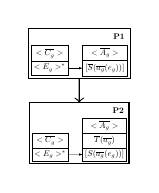
\begin{tikzpicture}[
single/.style={draw, anchor=text, rectangle},
double/.style={draw, anchor=text, rectangle split,rectangle split parts=2},
triple/.style={draw, anchor=text, rectangle split,rectangle split parts=3},
quadruple/.style={draw, anchor=text, rectangle split,rectangle split parts=4}
]
%% beginning of FIRST box
\node[single,scale=0.3] (first) at (0, 0) {
  \tikz{
%\draw[step=1cm,gray,very thin] (-4,-4) grid (4,4);
\node[double] (firstA) at (-2,0) {$<\overline{C_g}>$
  \nodepart{second}{$<E_g>^{*}$}
};
\node[double,right=6mm of firstA.east] (firstB) {$<\overline{A_g}>$
  \nodepart{second}{$[\overline{S}(\overline{a_g}(e_g))]$}
};
\draw [-latex] (firstA.two east) -- (firstB.two west);
\node[above = .01cm of firstB,label={[label distance=2mm]10:{\textbf{P1}}},inner sep=1pt]{};
}
};
%% end of first box

%% beginning of SECOND box
\node[single,scale=0.3,below=3mm of first, inner sep=1mm] (second) {
  \tikz{
%\draw[step=1cm,gray,very thin] (-4,-4) grid (4,4);
\node[double] (firstA) at (-2,0) {$<\overline{C_g}>$
  \nodepart{second}{$<E_g>^{*}$}
};
\node[triple,right=6mm of firstA.one east,yshift=.3mm] (firstB) {$<\overline{A_g}>$
  \nodepart{second}{$\overline{T}(\overline{a_g})$}
  \nodepart{third}{$[S(\overline{a_g}(e_g))]$}
};
\draw [-latex] (firstA.two east) -- (firstB.three west);
\node[above = .01cm of firstB,label={[label distance=2mm]10:{\textbf{P2}}},inner sep=1pt]{};
}
};;
%% end of second box

\draw[->] (first) -- (second);
\end{tikzpicture}}
\vspace{-5pt}
\caption{Progress in developing a poetry system\label{fig:poetry-progress}}
\vspace{-20pt}

\end{wrapfigure}
Progress amounts to more sophisticated processing, and, in the
notation, frequently corresponds to the removal of ``bars'' --
indicating that the system can do something that was formerly done by
a programmer.
%
Thus, this formalism keeps track both of the overall structure of
computational systems, and which actors that are responsible for which
actions within a given instance of the system.
%
As we develop models and systems that people would describe as
serendipitous with reference to the criteria listed in Section
\ref{sec:characteristics}, there will be more to account for.  

\smallskip

For example, we will need to model dynamically changing environments
and a computational version of a prepared mind.
%
To explore these features, are working with a system called {\sf
  FloWr}, portrayed with a screenshot in Figure \ref{fig:being-blunt}.
In {\sf FloWr}, users can construct complex flowcharts composed of
individual ProcessNodes, through which information flows and is
transformed.  The figure depicts a flowchart that has constructed a
poem based on live output from Twitter for the query ``blunt''.  The
dynamic aspects of this environment are threefold: (\emph{i}) some of
the nodes in the flowcharts access online news and social media sites,
which change rapidly from minute to minute; (\emph{ii}) the software
itself can construct new flowcharts, as described in
\cite{charnley2014flowr}; and (\emph{iii}) we are building a community
of ProcessNode builders around the online version of {\sf FloWr},
newly developed since the publication of \cite{charnley2014flowr} in
order to facilitate the direct involvement of other Computational
Creativity researchers.

\begin{figure}
\centering
\includegraphics[width=.95\textwidth]{being-blunt}
\caption{A sample poem generated by {\sf FloWr}\label{fig:being-blunt}}
\end{figure}


When {\sf FloWr} constructs flowcharts for itself, while each is
semantically plausible (i.e., they pass the right type of data from
ProcessNode to ProcessNode), many fail -- for instance, because the
available data is limited, or is narrowed down too quickly.  In fact,
the best results in \cite{charnley2014flowr} were at 20\%, i.e., 80\%
of the flowcharts that were constructed failed to produce output.
Each of these failures can be saved as an outstanding problem in {\sf
  FloWr}'s prepared mind.  As data changes and as new nodes are
written and uploaded to the system, {\sf FloWr} will be able to replace nodes,
update data sources, and in general rearrange flowcharts in order to
see if it can fix a broken flowchart.

For instance, suppose a ProcessNode developer wrote and uploaded a
node to mine data from a new social network, in order, say, to produce
textual summaries of world events.  {\sf FloWr} may take that node
and substitute it in the place of an old ``FaceBook'' node in a broken
poetry flowchart. If the replacement worked, and output was produced,
this could be seen as a serendipitous occurrence: {\sf FloWr} will
have taken advantage of the dynamically changing environment -- in
which new social networks come and go, and in which text summaries may
work better in some cases than in others -- to resolve an outstanding
problem in text generation.

The next stage for the {\sf FloWr} system will be to modify it along
these lines, to make it able to adapt to the dynamically changing
environment, and to perform experiments where we monitor potentially
serendipitous scenarios. Such experiments will be similar to those we
tried with the HR2 system in \cite{pease2013discussion}, but improved
because in this earlier effort, we had to break working processes in
order to serendipitously fix them.  The new experiments, the scenarios
will be more realistic, i.e., there will be a catalogue of genuine
open problems waiting to be solved.  Understanding how to work with
this catalogue and the associated experimental process will, of
course, be used to further the computational model of serendipity.  We
discuss one direction for such experiments in Section
\ref{sec:writers-workshop}.

\section{Patterns of Serendipity} \label{sec:patterns-of-serendipity}

\begin{figure}[p]
\centering
%\input{grid-input}
\resizebox{1.0\textwidth}{!}{%
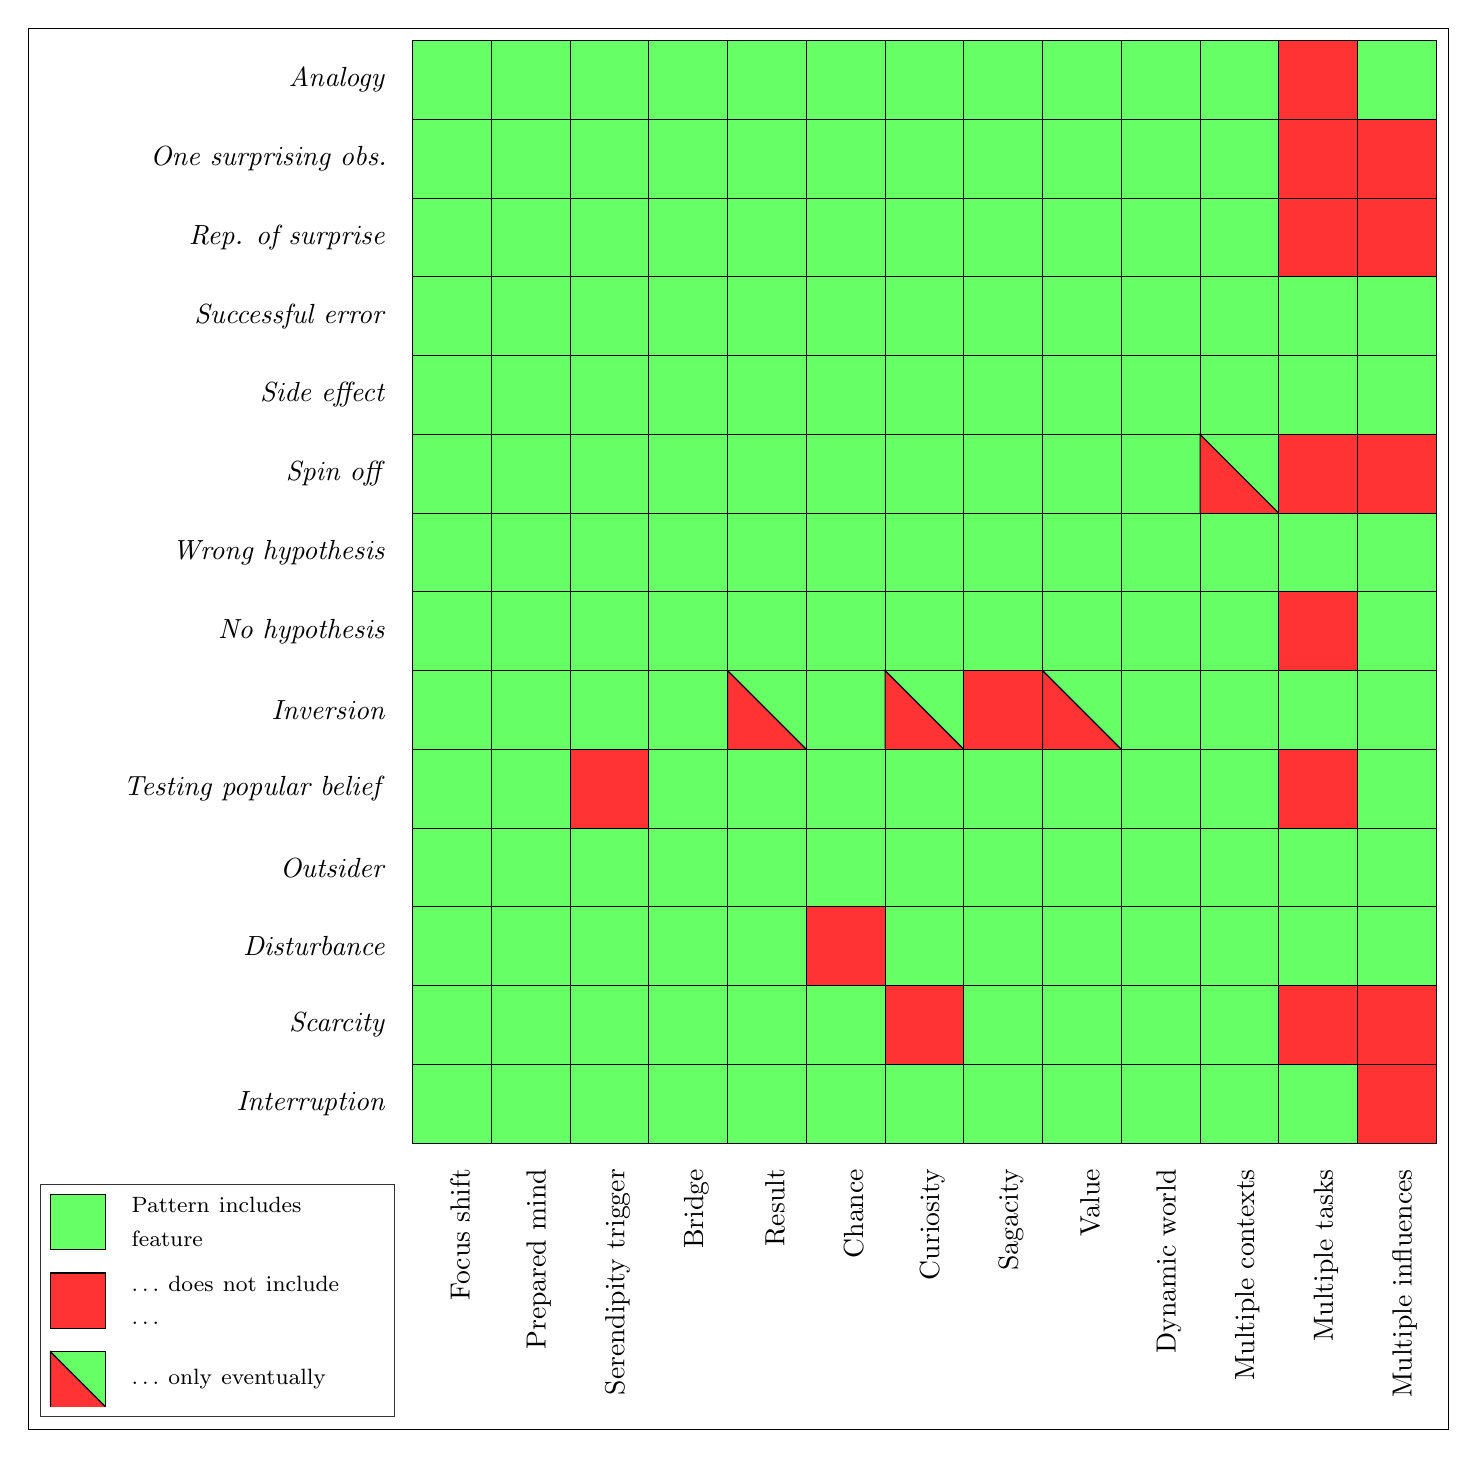
\begin{tikzpicture}[framed]
\draw[step=1cm,black,thin] (0,0) grid (12,13);
% Zeroth column
\node (bottom) at (-0.5,12.5)[draw,fill=green!60,minimum width=1cm,minimum height=1cm] {};  
\node[draw=none,left=.2cm of bottom.west,anchor=east] {\emph{Analogy}};
\node (bottom) at (-0.5,11.5)[draw,fill=green!60,minimum width=1cm,minimum height=1cm] {};  
\node[draw=none,left=.2cm of bottom.west,anchor=east] {\emph{One surprising obs.}};
\node (bottom) at (-0.5,10.5)[draw,fill=green!60,minimum width=1cm,minimum height=1cm] {};  
\node[draw=none,left=.2cm of bottom.west,anchor=east] {\emph{Rep. of surprise}};
\node (bottom) at (-0.5,9.5)[draw,fill=green!60,minimum width=1cm,minimum height=1cm] {};  
\node[draw=none,left=.2cm of bottom.west,anchor=east] {\emph{Successful error}}; 
\node (bottom) at (-0.5,8.5)[draw,fill=green!60,minimum width=1cm,minimum height=1cm] {};  
\node[draw=none,left=.2cm of bottom.west,anchor=east] {\emph{Side effect}};
\node (bottom) at (-0.5,7.5)[draw,fill=green!60,minimum width=1cm,minimum height=1cm] {};  
\node[draw=none,left=.2cm of bottom.west,anchor=east] {\emph{Spin off}};
\node (bottom) at (-0.5,6.5)[draw,fill=green!60,minimum width=1cm,minimum height=1cm] {};  
\node[draw=none,left=.2cm of bottom.west,anchor=east] {\emph{Wrong hypothesis}};
\node (bottom) at (-0.5,5.5)[draw,fill=green!60,minimum width=1cm,minimum height=1cm] {};  
\node[draw=none,left=.2cm of bottom.west,anchor=east] {\emph{No hypothesis}};
\node (bottom) at (-0.5,4.5)[draw,fill=green!60,minimum width=1cm,minimum height=1cm] {};  
\node[draw=none,left=.2cm of bottom.west,anchor=east] {\emph{Inversion}};
\node (bottom) at (-0.5,3.5)[draw,fill=green!60,minimum width=1cm,minimum height=1cm] {};  
\node[draw=none,left=.2cm of bottom.west,anchor=east] {\emph{Testing popular belief}};
\node (bottom) at (-0.5,2.5)[draw,fill=green!60,minimum width=1cm,minimum height=1cm] {};  
\node[draw=none,left=.2cm of bottom.west,anchor=east] {\emph{Outsider}};
\node (bottom) at (-0.5,1.5)[draw,fill=green!60,minimum width=1cm,minimum height=1cm] {};  
\node[draw=none,left=.2cm of bottom.west,anchor=east] {\emph{Disturbance}};
\node (bottom) at (-0.5,0.5)[draw,fill=green!60,minimum width=1cm,minimum height=1cm] {};  
\node[draw=none,left=.2cm of bottom.west,anchor=east] {\emph{Scarcity}}; 
\node (bottom) at (-0.5,-0.5)[draw,fill=green!60,minimum width=1cm,minimum height=1cm] {};  
\node[draw=none,left=.2cm of bottom.west,anchor=east] {\emph{Interruption}};
\node[draw=none,rotate=90,below=.2cm of bottom.south,yshift=-.1cm,anchor=east] {Focus shift};
% First column
\node (bottom) at (0.5,12.5)[draw,fill=green!60,minimum width=1cm,minimum height=1cm] {};  
\node (bottom) at (0.5,11.5)[draw,fill=green!60,minimum width=1cm,minimum height=1cm] {};  
\node (bottom) at (0.5,10.5)[draw,fill=green!60,minimum width=1cm,minimum height=1cm] {};  
\node (bottom) at (0.5,9.5)[draw,fill=green!60,minimum width=1cm,minimum height=1cm] {};  
\node (bottom) at (0.5,8.5)[draw,fill=green!60,minimum width=1cm,minimum height=1cm] {};  
\node (bottom) at (0.5,7.5)[draw,fill=green!60,minimum width=1cm,minimum height=1cm] {};  
\node (bottom) at (0.5,6.5)[draw,fill=green!60,minimum width=1cm,minimum height=1cm] {};  
\node (bottom) at (0.5,5.5)[draw,fill=green!60,minimum width=1cm,minimum height=1cm] {};  
\node (bottom) at (0.5,4.5)[draw,fill=green!60,minimum width=1cm,minimum height=1cm] {};  
\node (bottom) at (0.5,3.5)[draw,fill=green!60,minimum width=1cm,minimum height=1cm] {};  
\node (bottom) at (0.5,2.5)[draw,fill=green!60,minimum width=1cm,minimum height=1cm] {};  
\node (bottom) at (0.5,1.5)[draw,fill=green!60,minimum width=1cm,minimum height=1cm] {};  
\node (bottom) at (0.5,0.5)[draw,fill=green!60,minimum width=1cm,minimum height=1cm] {};  
\node (bottom) at (0.5,-0.5)[draw,fill=green!60,minimum width=1cm,minimum height=1cm] {};  
\node[draw=none,rotate=90,below=.2cm of bottom.south,yshift=-.1cm,anchor=east] {Prepared mind};
 % Interruption               
% Second column
\node at (1.5,12.5) [draw,fill=green!60,minimum width=1cm,minimum height=1cm]{};
\node at (1.5,11.5) [draw,fill=green!60,minimum width=1cm,minimum height=1cm]{};
\node at (1.5,10.5) [draw,fill=green!60,minimum width=1cm,minimum height=1cm]{};
\node at (1.5,9.5)  [draw,fill=green!60,minimum width=1cm,minimum height=1cm]{};
\node at (1.5,8.5)  [draw,fill=green!60,minimum width=1cm,minimum height=1cm]{};
\node at (1.5,7.5)  [draw,fill=green!60,minimum width=1cm,minimum height=1cm]{};
\node at (1.5,6.5)  [draw,fill=green!60,minimum width=1cm,minimum height=1cm]{};
\node at (1.5,5.5)  [draw,fill=green!60,minimum width=1cm,minimum height=1cm]{};
\node at (1.5,4.5)  [draw,fill=green!60,minimum width=1cm,minimum height=1cm]{};
\node at (1.5,3.5)  [draw,fill=red!80,minimum width=1cm,minimum height=1cm]{};
\node at (1.5,2.5)  [draw,fill=green!60,minimum width=1cm,minimum height=1cm]{};
\node at (1.5,1.5)  [draw,fill=green!60,minimum width=1cm,minimum height=1cm]{};
\node at (1.5,0.5)  [draw,fill=green!60,minimum width=1cm,minimum height=1cm]{};
\node (bottom) at (1.5,-0.5)[draw,fill=green!60,minimum width=1cm,minimum height=1cm] {};  
\node[draw=none,rotate=90,below=.2cm of bottom.south,yshift=-.1cm,anchor=east] {Serendipity trigger};
% Third column
\node at (2.5,12.5) [draw,fill=green!60,minimum width=1cm,minimum height=1cm]{}; % Analogy                    
\node at (2.5,11.5) [draw,fill=green!60,minimum width=1cm,minimum height=1cm]{}; % One surprising observation 
\node at (2.5,10.5) [draw,fill=green!60,minimum width=1cm,minimum height=1cm]{}; % Repetition of surprise     
\node at (2.5,9.5)  [draw,fill=green!60,minimum width=1cm,minimum height=1cm]{}; % Successful error           
\node at (2.5,8.5)  [draw,fill=green!60,minimum width=1cm,minimum height=1cm]{}; % Side effect                
\node at (2.5,7.5)  [draw,fill=green!60,minimum width=1cm,minimum height=1cm]{}; % Spin off                   
\node at (2.5,6.5)  [draw,fill=green!60,minimum width=1cm,minimum height=1cm]{}; % Wrong hypothesis           
\node at (2.5,5.5)  [draw,fill=green!60,minimum width=1cm,minimum height=1cm]{}; % No hypothesis              
\node at (2.5,4.5)  [draw,fill=green!60,minimum width=1cm,minimum height=1cm]{}; % Inversion                  
\node at (2.5,3.5)  [draw,fill=green!60,minimum width=1cm,minimum height=1cm]{}; % Testing popular belief     
\node at (2.5,2.5)  [draw,fill=green!60,minimum width=1cm,minimum height=1cm]{}; % outsider    
\node at (2.5,1.5)  [draw,fill=green!60,minimum width=1cm,minimum height=1cm]{}; % Disturbance                
\node at (2.5,0.5)  [draw,fill=green!60,minimum width=1cm,minimum height=1cm]{}; % Scarcity                   
\node (bottom) at (2.5,-0.5)[draw,fill=green!60,minimum width=1cm,minimum height=1cm] {};  
\node[draw=none,rotate=90,below=.2cm of bottom.south,yshift=-.1cm,anchor=east] {Bridge};
% Fourth column
\node at (3.5,12.5) [draw,fill=green!60,minimum width=1cm,minimum height=1cm]{}; % Analogy                    
\node at (3.5,11.5) [draw,fill=green!60,minimum width=1cm,minimum height=1cm]{}; % One surprising observation 
\node at (3.5,10.5) [draw,fill=green!60,minimum width=1cm,minimum height=1cm]{}; % Repetition of surprise     
\node at (3.5,9.5)  [draw,fill=green!60,minimum width=1cm,minimum height=1cm]{}; % Successful error           
\node at (3.5,8.5)  [draw,fill=green!60,minimum width=1cm,minimum height=1cm]{}; % Side effect                
\node at (3.5,7.5)  [draw,fill=green!60,minimum width=1cm,minimum height=1cm]{}; % Spin off                   
\node at (3.5,6.5)  [draw,fill=green!60,minimum width=1cm,minimum height=1cm]{}; % Wrong hypothesis           
\node at (3.5,5.5)  [draw,fill=green!60,minimum width=1cm,minimum height=1cm]{}; % No hypothesis              
\node at (3.5,4.5)  [draw,fill=green!60,minimum width=1cm,minimum height=1cm]{}; % Inversion
\draw [fill=red!80] (3,4) -- (3,5) -- (4,4);  
\node at (3.5,3.5)  [draw,fill=green!60,minimum width=1cm,minimum height=1cm]{}; % Testing popular belief     
\node at (3.5,2.5)  [draw,fill=green!60,minimum width=1cm,minimum height=1cm]{}; % Outsider
\node at (3.5,1.5)  [draw,fill=green!60,minimum width=1cm,minimum height=1cm]{}; % Disturbance                
\node at (3.5,0.5)  [draw,fill=green!60,minimum width=1cm,minimum height=1cm]{}; % Scarcity                   
%\node at (3,0)  [draw,fill=green!60,minimum width=1cm,minimum height=1cm]{}; % Interruption               
\node (bottom) at (3.5,-0.5)[draw,fill=green!60,minimum width=1cm,minimum height=1cm] {};  
\node[draw=none,rotate=90,below=.2cm of bottom.south,yshift=-.1cm,anchor=east] {Result};
% Fifth column
\node at (4.5,12.5) [draw,fill=green!60,minimum width=1cm,minimum height=1cm]{}; % Analogy                    
\node at (4.5,11.5) [draw,fill=green!60,minimum width=1cm,minimum height=1cm]{}; % One surprising observation 
\node at (4.5,10.5) [draw,fill=green!60,minimum width=1cm,minimum height=1cm]{}; % Repetition of surprise     
\node at (4.5,9.5)  [draw,fill=green!60,minimum width=1cm,minimum height=1cm]{}; % Successful error           
\node at (4.5,8.5)  [draw,fill=green!60,minimum width=1cm,minimum height=1cm]{}; % Side effect                
\node at (4.5,7.5)  [draw,fill=green!60,minimum width=1cm,minimum height=1cm]{}; % Spin off                   
\node at (4.5,6.5)  [draw,fill=green!60,minimum width=1cm,minimum height=1cm]{}; % Wrong hypothesis           
\node at (4.5,5.5)  [draw,fill=green!60,minimum width=1cm,minimum height=1cm]{}; % No hypothesis              
\node at (4.5,4.5)  [draw,fill=green!60,minimum width=1cm,minimum height=1cm]{}; % Inversion
\node at (4.5,3.5)  [draw,fill=green!60,minimum width=1cm,minimum height=1cm]{}; % Testing popular belief     
\node at (4.5,2.5)  [draw,fill=green!60,minimum width=1cm,minimum height=1cm]{}; % Testing popular belief     
\node at (4.5,1.5)  [draw,fill=red!80,minimum width=1cm,minimum height=1cm]{}; % Disturbance                
\node at (4.5,0.5)  [draw,fill=green!60,minimum width=1cm,minimum height=1cm]{}; % Scarcity                   
% \node at (4,0)  [draw,fill=green!60,minimum width=1cm,minimum height=1cm]{}; % Interruption               
\node (bottom) at (4.5,-0.5)[draw,fill=green!60,minimum width=1cm,minimum height=1cm] {};  
\node[draw=none,rotate=90,below=.2cm of bottom.south,yshift=-.1cm,anchor=east] {Chance};
% Sixth column
\node at (5.5,12.5) [draw,fill=green!60,minimum width=1cm,minimum height=1cm]{}; % Analogy                    
\node at (5.5,11.5) [draw,fill=green!60,minimum width=1cm,minimum height=1cm]{}; % One surprising observation 
\node at (5.5,10.5) [draw,fill=green!60,minimum width=1cm,minimum height=1cm]{}; % Repetition of surprise     
\node at (5.5,9.5)  [draw,fill=green!60,minimum width=1cm,minimum height=1cm]{}; % Successful error           
\node at (5.5,8.5)  [draw,fill=green!60,minimum width=1cm,minimum height=1cm]{}; % Side effect                
\node at (5.5,7.5)  [draw,fill=green!60,minimum width=1cm,minimum height=1cm]{}; % Spin off                   
\node at (5.5,6.5)  [draw,fill=green!60,minimum width=1cm,minimum height=1cm]{}; % Wrong hypothesis           
\node at (5.5,5.5)  [draw,fill=green!60,minimum width=1cm,minimum height=1cm]{}; % No hypothesis              
\node at (5.5,4.5)  [draw,fill=green!60,minimum width=1cm,minimum height=1cm]{}; % Inversion                  
\draw [fill=red!80] (5,4) -- (5,5) -- (6,4);  
\node at (5.5,3.5)  [draw,fill=green!60,minimum width=1cm,minimum height=1cm]{}; % Testing popular belief     
\node at (5.5,2.5)  [draw,fill=green!60,minimum width=1cm,minimum height=1cm]{}; % Testing popular belief     
\node at (5.5,1.5)  [draw,fill=green!60,minimum width=1cm,minimum height=1cm]{}; % Disturbance                
\node at (5.5,0.5)  [draw,fill=red!80,minimum width=1cm,minimum height=1cm]{}; % Scarcity                   
% \node at (5,0)  [draw,fill=green!60,minimum width=1cm,minimum height=1cm]{}; % Interruption               
\node (bottom) at (5.5,-0.5)[draw,fill=green!60,minimum width=1cm,minimum height=1cm] {};  
\node[draw=none,rotate=90,below=.2cm of bottom.south,yshift=-.1cm,anchor=east] {Curiosity};
% Seventh column
\node at (6.5,12.5) [draw,fill=green!60,minimum width=1cm,minimum height=1cm]{}; % Analogy                    
\node at (6.5,11.5) [draw,fill=green!60,minimum width=1cm,minimum height=1cm]{}; % One surprising observation 
\node at (6.5,10.5) [draw,fill=green!60,minimum width=1cm,minimum height=1cm]{}; % Repetition of surprise     
\node at (6.5,9.5)  [draw,fill=green!60,minimum width=1cm,minimum height=1cm]{}; % Successful error           
\node at (6.5,8.5)  [draw,fill=green!60,minimum width=1cm,minimum height=1cm]{}; % Side effect                
\node at (6.5,7.5)  [draw,fill=green!60,minimum width=1cm,minimum height=1cm]{}; % Spin off                   
\node at (6.5,6.5)  [draw,fill=green!60,minimum width=1cm,minimum height=1cm]{}; % Wrong hypothesis           
\node at (6.5,5.5)  [draw,fill=green!60,minimum width=1cm,minimum height=1cm]{}; % No hypothesis              
\node at (6.5,4.5)  [draw,fill=red!80,minimum width=1cm,minimum height=1cm]{}; % Inversion                  
\node at (6.5,3.5)  [draw,fill=green!60,minimum width=1cm,minimum height=1cm]{}; % Testing popular belief     
\node at (6.5,2.5)  [draw,fill=green!60,minimum width=1cm,minimum height=1cm]{}; % Testing popular belief     
\node at (6.5,1.5)  [draw,fill=green!60,minimum width=1cm,minimum height=1cm]{}; % Disturbance                
\node at (6.5,0.5)  [draw,fill=green!60,minimum width=1cm,minimum height=1cm]{}; % Scarcity                   
% \node at (6,0)  [draw,fill=green!60,minimum width=1cm,minimum height=1cm]{}; % Interruption               
\node (bottom) at (6.5,-0.5)[draw,fill=green!60,minimum width=1cm,minimum height=1cm] {};  
\node[draw=none,rotate=90,below=.2cm of bottom.south,yshift=-.1cm,anchor=east] {Sagacity};
% Eighth column
\node at (7.5,12.5) [draw,fill=green!60,minimum width=1cm,minimum height=1cm]{}; % Analogy                    
\node at (7.5,11.5) [draw,fill=green!60,minimum width=1cm,minimum height=1cm]{}; % One surprising observation 
\node at (7.5,10.5) [draw,fill=green!60,minimum width=1cm,minimum height=1cm]{}; % Repetition of surprise     
\node at (7.5,9.5)  [draw,fill=green!60,minimum width=1cm,minimum height=1cm]{}; % Successful error           
\node at (7.5,8.5)  [draw,fill=green!60,minimum width=1cm,minimum height=1cm]{}; % Side effect                
\node at (7.5,7.5)  [draw,fill=green!60,minimum width=1cm,minimum height=1cm]{}; % Spin off                   
\node at (7.5,6.5)  [draw,fill=green!60,minimum width=1cm,minimum height=1cm]{}; % Wrong hypothesis           
\node at (7.5,5.5)  [draw,fill=green!60,minimum width=1cm,minimum height=1cm]{}; % No hypothesis              
%\node at (7.5,4.5)  [draw,shading=axis,bottom color=green!60,top color=red,minimum width=1cm,minimum height=1cm,shading angle=45]{}; % Inversion
\node at (7.5,4.5)  [draw,fill=green!60,minimum width=1cm,minimum height=1cm]{}; % Inversion
%% half off
\draw [fill=red!80] (7,4) -- (7,5) -- (8,4);  % Interruption
%\draw (7,4) -- (8,5);  % Interruption
\node at (7.5,3.5)  [draw,fill=green!60,minimum width=1cm,minimum height=1cm]{}; % Testing popular belief     
\node at (7.5,2.5)  [draw,fill=green!60,minimum width=1cm,minimum height=1cm]{}; % outsider
\node at (7.5,1.5)  [draw,fill=green!60,minimum width=1cm,minimum height=1cm]{}; % Disturbance                
\node at (7.5,0.5)  [draw,fill=green!60,minimum width=1cm,minimum height=1cm]{}; % Scarcity                   
%\node at (7,0)  [draw,fill=green!60,minimum width=1cm,minimum height=1cm]{}; % Interruption               
\node (bottom) at (7.5,-0.5)[draw,fill=green!60,minimum width=1cm,minimum height=1cm] {};  
\node[draw=none,rotate=90,below=.2cm of bottom.south,yshift=-.1cm,anchor=east] {Value};
%%%%%%%%%%%%%%%
% Ninth column
\node at (8.5,12.5) [draw,fill=green!60,minimum width=1cm,minimum height=1cm]{}; % Analogy                    
\node at (8.5,11.5) [draw,fill=green!60,minimum width=1cm,minimum height=1cm]{}; % One surprising observation 
\node at (8.5,10.5) [draw,fill=green!60,minimum width=1cm,minimum height=1cm]{}; % Repetition of surprise     
\node at (8.5,9.5)  [draw,fill=green!60,minimum width=1cm,minimum height=1cm]{}; % Successful error           
\node at (8.5,8.5)  [draw,fill=green!60,minimum width=1cm,minimum height=1cm]{}; % Side effect                
\node at (8.5,7.5)  [draw,fill=green!60,minimum width=1cm,minimum height=1cm]{}; % Spin off                   
\node at (8.5,6.5)  [draw,fill=green!60,minimum width=1cm,minimum height=1cm]{}; % Wrong hypothesis           
\node at (8.5,5.5)  [draw,fill=green!60,minimum width=1cm,minimum height=1cm]{}; % No hypothesis              
\node at (8.5,4.5)  [draw,fill=green!60,minimum width=1cm,minimum height=1cm]{}; % Inversion                  
\node at (8.5,3.5)  [draw,fill=green!60,minimum width=1cm,minimum height=1cm]{}; % Testing popular belief     
\node at (8.5,2.5)  [draw,fill=green!60,minimum width=1cm,minimum height=1cm]{}; % Testing popular belief     
\node at (8.5,1.5)  [draw,fill=green!60,minimum width=1cm,minimum height=1cm]{}; % Disturbance                
\node at (8.5,0.5)  [draw,fill=green!60,minimum width=1cm,minimum height=1cm]{}; % Scarcity                   
% \node at (8,0)  [draw,fill=green!60,minimum width=1cm,minimum height=1cm]{}; % Interruption               
\node (bottom) at (8.5,-0.5)[draw,fill=green!60,minimum width=1cm,minimum height=1cm] {};  
\node[draw=none,rotate=90,below=.2cm of bottom.south,yshift=-.1cm,anchor=east] {Dynamic world};
% Tenth column
\node at (9.5,12.5) [draw,fill=green!60,minimum width=1cm,minimum height=1cm]{}; % Analogy                    
\node at (9.5,11.5) [draw,fill=green!60,minimum width=1cm,minimum height=1cm]{}; % One surprising observation 
\node at (9.5,10.5) [draw,fill=green!60,minimum width=1cm,minimum height=1cm]{}; % Repetition of surprise     
\node at (9.5,9.5)  [draw,fill=green!60,minimum width=1cm,minimum height=1cm]{}; % Successful error           
\node at (9.5,8.5)  [draw,fill=green!60,minimum width=1cm,minimum height=1cm]{}; % Side effect                
\node at (9.5,7.5)  [draw,fill=green!60,minimum width=1cm,minimum height=1cm]{}; % Spin off
\draw [fill=red!80] (9,7) -- (9,8) -- (10,7);  
\node at (9.5,6.5)  [draw,fill=green!60,minimum width=1cm,minimum height=1cm]{}; % Wrong hypothesis           
\node at (9.5,5.5)  [draw,fill=green!60,minimum width=1cm,minimum height=1cm]{}; % No hypothesis              
\node at (9.5,4.5)  [draw,fill=green!60,minimum width=1cm,minimum height=1cm]{}; % Inversion                  
\node at (9.5,3.5)  [draw,fill=green!60,minimum width=1cm,minimum height=1cm]{}; % Testing popular belief     
\node at (9.5,2.5)  [draw,fill=green!60,minimum width=1cm,minimum height=1cm]{}; % Testing popular belief     
\node at (9.5,1.5)  [draw,fill=green!60,minimum width=1cm,minimum height=1cm]{}; % Disturbance                
\node at (9.5,0.5)  [draw,fill=green!60,minimum width=1cm,minimum height=1cm]{}; % Scarcity                   
% \node at (9,0)  [draw,fill=green!60,minimum width=1cm,minimum height=1cm]{}; % Interruption               
\node (bottom) at (9.5,-0.5)[draw,fill=green!60,minimum width=1cm,minimum height=1cm] {};  
\node[draw=none,rotate=90,below=.2cm of bottom.south,yshift=-.1cm,anchor=east] {Multiple contexts};
% Eleventh column
\node at (10.5,12.5) [draw,fill=red!80,minimum width=1cm,minimum height=1cm]{}; % Analogy                    
\node at (10.5,11.5) [draw,fill=red!80,minimum width=1cm,minimum height=1cm]{}; % One surprising observation 
\node at (10.5,10.5) [draw,fill=red!80,minimum width=1cm,minimum height=1cm]{}; % Repetition of surprise     
\node at (10.5,9.5)  [draw,fill=green!60,minimum width=1cm,minimum height=1cm]{}; % Successful error           
\node at (10.5,8.5)  [draw,fill=green!60,minimum width=1cm,minimum height=1cm]{}; % Side effect                
\node at (10.5,7.5)  [draw,fill=red!80,minimum width=1cm,minimum height=1cm]{}; % Spin off                   
\node at (10.5,6.5)  [draw,fill=green!60,minimum width=1cm,minimum height=1cm]{}; % Wrong hypothesis           
\node at (10.5,5.5)  [draw,fill=red!80,minimum width=1cm,minimum height=1cm]{}; % No hypothesis              
\node at (10.5,4.5)  [draw,fill=green!60,minimum width=1cm,minimum height=1cm]{}; % Inversion                  
\node at (10.5,3.5)  [draw,fill=red!80,minimum width=1cm,minimum height=1cm]{}; % Testing popular belief     
\node at (10.5,2.5)  [draw,fill=green!60,minimum width=1cm,minimum height=1cm]{}; % outsider
\node at (10.5,1.5)  [draw,fill=green!60,minimum width=1cm,minimum height=1cm]{}; % Disturbance                
\node at (10.5,0.5)  [draw,fill=red!80,minimum width=1cm,minimum height=1cm]{}; % Scarcity                   
% \node at (10,0)  [draw,fill=green!60,minimum width=1cm,minimum height=1cm]{}; % Interruption               
\node (bottom) at (10.5,-0.5)[draw,fill=green!60,minimum width=1cm,minimum height=1cm] {};  
\node[draw=none,rotate=90,below=.2cm of bottom.south,yshift=-.1cm,anchor=east] {Multiple tasks};
% Twelfth column
\node at (11.5,12.5) [draw,fill=green!60,minimum width=1cm,minimum height=1cm]{}; % Analogy                    
\node at (11.5,11.5) [draw,fill=red!80,minimum width=1cm,minimum height=1cm]{}; % One surprising observation 
\node at (11.5,10.5) [draw,fill=red!80,minimum width=1cm,minimum height=1cm]{}; % Repetition of surprise     
\node at (11.5,9.5)  [draw,fill=green!60,minimum width=1cm,minimum height=1cm]{}; % Successful error           
\node at (11.5,8.5)  [draw,fill=green!60,minimum width=1cm,minimum height=1cm]{}; % Side effect                
\node at (11.5,7.5)  [draw,fill=red!80,minimum width=1cm,minimum height=1cm]{}; % Spin off                   
\node at (11.5,6.5)  [draw,fill=green!60,minimum width=1cm,minimum height=1cm]{}; % Wrong hypothesis           
\node at (11.5,5.5)  [draw,fill=green!60,minimum width=1cm,minimum height=1cm]{}; % No hypothesis              
\node at (11.5,4.5)  [draw,fill=green!60,minimum width=1cm,minimum height=1cm]{}; % Inversion                  
\node at (11.5,3.5)  [draw,fill=green!60,minimum width=1cm,minimum height=1cm]{}; % Testing popular belief     
\node at (11.5,2.5)  [draw,fill=green!60,minimum width=1cm,minimum height=1cm]{}; % Testing popular belief     
\node at (11.5,1.5)  [draw,fill=green!60,minimum width=1cm,minimum height=1cm]{}; % Disturbance                
\node at (11.5,0.5)  [draw,fill=red!80,minimum width=1cm,minimum height=1cm]{}; % Scarcity                   
\node (bottom) at (11.5,-0.5)[draw,fill=red!80,minimum width=1cm,minimum height=1cm] {};  
\node[draw=none,rotate=90,below=.2cm of bottom.south,yshift=-.1cm,anchor=east] {Multiple influences};

\begin{scope}[xshift=.5cm,yshift=0cm]
\node (A) at (-5.75,-2.0)  [draw,fill=green!60,minimum width=.7cm,minimum height=.7cm]{}; %
\node[draw=none,right=.2cm of A.east,text width=3.10cm] {{\footnotesize Pattern includes\par feature}}; 
\node (B) at (-5.75,-3.0)  [draw,fill=red!80,minimum width=.7cm,minimum height=.7cm]{}; %
\node[draw=none,right=.2cm of B.east,text width=3.10cm] {{\footnotesize $\ldots$ does not include $\ldots$}}; 

\node (C) at (-5.75,-4)  [draw,fill=green!60,minimum width=.7cm,minimum height=.7cm]{}; %
\node[draw=none,right=.2cm of C.east,text width=3.10cm] (Ct) {{\footnotesize $\ldots$ only eventually}};
%% half off
\draw [fill=red!80] (-6.1,-4.35) -- (-6.1,-3.65) -- (-5.4,-4.35);  

\node[draw=black!80, fit=(A) (B) (C) (Ct)](FIt1) {};
\end{scope}
\end{tikzpicture}
}
\caption{Characteristics of Pek van Andel's patterns of serendipity\label{fig:grid}}
\end{figure}

% ***AJ what is a 'situational pattern of serendipity'? Can we add a definition e.g. from van Andel***
Figure \ref{fig:grid} examines 14 situational patterns of serendipity
collected by van Andel \cite{van1994anatomy} through the lens of the evaluation
criteria described in Section \ref{sec:literature-review}.
%
As required by our theory, a ``focus shift'' appears in each instance,
although it has a different flavour in the different examples.  In
this analysis, only three of the other criteria mentioned above are
clearly present in \emph{all} of the patterns: ``a prepared mind'', a
``bridge'', and a ``dynamic world.''  Similarly, only four of van
Andel's patterns exhibit all of the characteristics we identified:
\emph{Successful error}, \emph{Side effect}, \emph{Wrong hypothesis},
and \emph{Outsider}.

``Near misses'' are also of interest, and help to illustrate the role
of the various factors from Section \ref{sec:literature-review}.
%
For example, the \emph{Inversion} pattern is somewhat closer to what is called an \emph{antipattern} in the design pattern literature \cite{brown1998antipatterns}.  Van Andel describes the story of a researcher observing an effect (the anticoagulant heparine) which was precisely the opposite of the one sought (factors that \emph{cause} blood clotting) -- and failing to acknowledge that this observation was important for over 40 years.  The result was eventually seen to be of value: however, in this instance, we may have an example of a mind that is \emph{over-prepared}, and focused on a particular sort of result, rather than a truly ``sagacious'' mind that is both prepared and open to serendipitous findings.

In the case of \emph{Testing popular belief}, van Andel gives an
account of a medical practise that originated in a folk claim, namely
cowpox-derived immunity to smallpox.  This effect, for milkmaids,
might indeed be called serendipitous.  Indeed, the medical use of
cowpox has been described as ``widely know'' \cite{riedel2005edward}
prior to its popularisation by Edward Jenner.  Nevertheless, 
Jenner's ``relentless promotion and devoted research of vaccination
\ldots changed the way medicine was practised'' \cite{riedel2005edward}.
This again might be called serendipity, but most clearly at the social
rather than personal level.  These comments should not be seen to
disparage Jenner's contribution, or diminish the role of a curious
chain of events in his personal history that tied his fate to that of
the smallpox vaccine.  Many of these had the air of serendipity about
them -- but even so, it is hard to find one specific ``serendipity
trigger.''
 
In describing \emph{Disturbance}, van Andel's exemplar is the
creation of radio telescopy from noise in transatlantic telephone calls
(paralleling the subsequent discovery by Penzias and Wilson).  Here it
is hard to see an overt role for ``chance,'' since as machinery at
various scales is created, disturbance is somewhat inevitable, even if
a specific disturbance in a specific machine is unexpected.
Similarly, in cases of \emph{Scarcity}, ``curiosity'' may not play a
significant role, and may instead be replaced by the drive of desire
and corresponding ingenuity.

Multiple contexts, tasks, and influences should be seen to be
conducive to serendipitous discovery, but not strictly necessary.  For
example, in addition to the context of a research laboratory, there
may be the context of subsequent industrial application.  However,
within the laboratory itself (where a \emph{Spin off} discovery might
be made) the future context is not typically in force.

There are a number of additional reoccurring themes, which are worthy
of further comment, and which could form the basis of further
(meta-)patterns.

\begin{description}
\item[\emph{It's all part of a day's work.}] Often the discoverer had
  a problem to solve or job to do, and made the serendipitous
  discovery in the course of doing their job.  This sort of
  serendipity is often ``social.''  For example, in the
  \emph{Outsider} pattern, the ophthalmologist Gregg was simply
  listening to his patient and taking what she said seriously; in
  other words, he was doing his job.  But this led to a new
  hypothesis.
\item[\emph{Factorisation is useful.}] Variability, and in the case of
  scientific work, factorisation (e.g. via control studies) often
  plays a key role in establishing ``multiple contexts.''
  Serendipitous discovery often happens in the context of ``natural
  experiments,'' for example, in the case of \emph{One surprising
    observation}, where van Andel's example dealt with the observation
  that one tree in a row was taller and healthier than its
  neighbours.\footnote{Concerning the broader issues associated with
    the ``design'' of such experiments, see
    \cite{imbens1994identification}.}
\item[\emph{A good story is liable to change.}] Comparing
  \emph{Inversion} and \emph{Spin off} suggests the value of being
  able to change the story.  If Perkin had suppressed his discovery of
  mauvine because he hadn't successfully synthesised quinine, there
  would have been no spin off, and it would be hard to call the
  discovery ``serendipitous'' -- or, indeed, to consider it to be a
  discovery at all.  Whatever its value, an event may only be
  \emph{described} as serendipitous at the narrative level.
\item[\emph{Watch out for hidden symmetries.}] The \emph{Wrong
  hypothesis} pattern involves several of the points above.  In van
  Andel's anecdote about John Cade's discovery of lithium as a
  \emph{treatment} for mania, the issues under investigation were,
  rather, the \emph{causes} of the illness.  This was initially
  conceptualised in terms of \emph{surfeit} and \emph{deficiency}.  A
  more general interpretation is that the factors influencing the
  course of an illness have hidden interactions between them.
  Serendipitous discovery may be able to find and capitalise on this
  type of (unexpected) invariant.
\end{description}

Van Andel describes three additional patterns that seem to be
connected with personal qualities of the investigator rather than with
situational features.  These are \emph{Playing}, \emph{Joke}, and
\emph{Dream}.  The theme of personal qualities and skills that support
serendipitous discovery will be taken up below, as part of a general
approach to modelling serendipity.

\subsection{Modelling serendipity with design patterns} \label{sec:unified-approach}

As illustrated above, serendipity can take place on multiple scales.
Something can be personally surprising while being socially mundane
(Boden's \emph{P-creativity} \cite{boden}), or vice versa, as in
the case of personally mundane discoveries that take on surprising
social value.

In the case of serendipitous discoveries at the personal level, the
qualities of the investigator are understood to be important features.
Thus, for example, van Andel writes that a ``sense of humour and
  sense of serendipity have a lot in common.'' 
% 
Van Andel relates the \emph{Dream} pattern -- exemplified, for him by
Descartes, but Kekul\'e's ouroborus provides another instance -- to
Poincar\'e's \cite{poincare1910creation,poincare2013science} model of
``preparation, incubation, illumination, and verification''
(cf. \cite{wallas1926art}).  Poincar\'e \cite{poincare1910creation}
clarifies that
\begin{quote}
``\emph{unconscious work}~\ldots~\emph{is possible, and of a
    certainty, it is only fruitful, if it is on the one hand preceded
    and on the other hand followed by a period of conscious work.}''
\end{quote}

What might conceptions like this mean for serendipity that takes place
on a social or indeed computational level?  In order to understand
this, we will refer van Andel's patterns and the serendipity factors
introduced above to the heterodox theory of patterns coming from the
field of design, mentioned briefly above.  First introduced by the
architect Christopher Alexander
\cite{alexander1979timeless,alexander1977pattern}, the design pattern
methodology spread from architecture to software
\cite{gabriel1996patterns}, and later, to other fields, including
public affairs \cite{schuler2008liberating} and education
\cite{bergin2012pedagogical}.

Alexander's patterns are presented in a tree-like structure called a
\emph{pattern language}, ordered in a top-down manner from large-scale
to small-scale levels of application, with each pattern presented in
terms of a \emph{picture}, a \emph{context} (including links to
relevant larger patterns), the \emph{problem} that the pattern
addresses, the \emph{solution}, a \emph{diagram}, and \emph{links to
  smaller patterns} \cite[pp. x-xi]{alexander1977pattern}.
%
A relatively convincing implementation of
Alexander's idea of patterns as a ``living
  language''
\cite[p. xvii]{alexander1977pattern} was realised
with one of the earliest applications of wiki
software developed by Ward Cunningham: the
Portland Pattern
Repository.\footnote{\url{http://c2.com/ppr/}}
The notion of pattern-finding as a process
related to, but distinct from abstraction, is
described by Richard Gabriel, who emphasises that
the ``patterns and the social process for
  applying them are designed to produce organic
  order through piecemeal growth''
\cite[p. 31]{gabriel1996patterns}.
%
In its original form, this statement describes the generative use of
patterns to create artefacts (buildings, object oriented programs,
etc.).  However, this criterion can also be applied to the growth and
development the pattern language itself, and this is the key idea
underlying our application.

Christian Kohls \cite{kohls2010structure,kohls2011structure}, deploys
a ``path'' or ``journey'' metaphor to describe design patterns in the
language of constrained optimisation problems, considering in
particular the \emph{initial state}, \emph{end state}, and
\emph{forces acting}.  This is useful because of its general nature:
it suggests that any time there are predictable dynamics observed in
the world, there is a corresponding design pattern waiting to be seen
and recorded.  This perspective can be usefully combined with the
proposal advanced by Manual DeLanda \cite{delanda2011philosophy},
among others, to give the system a simulated embodiment, putting it in
contact with a virtual world in which it does not need to, and indeed
cannot, have everything worked out in advance.  DeLanda uses the term
\emph{gradient} to describe the forces acting in a way that focuses on
the relevant features.  Like Kohls, Peter Andersen
\cite{andersen2002dynamic} considers one-dimensional paths through a
two-dimensional space with a gradient, and writes that the basic
metaphor for thought is travel.  A more general metaphor suggested
by DeLanda would take into account
%
``a population of interacting physical entities, such as the molecules
in a thin layer of soap'' \cite{delanda2005deleuze} exhibiting more
complex non-linear interactions over higher-dimensional gradients.

This discussion makes a distinction between an agential system of
interest and its broader context, which could also be described as a
physical ``system,'' or a simulation of one.  While such distinctions
tend to be leaky, to avoid undo confusion about terminology, when we
refer to ``the system'' without further qualification, we mean the
agential sub-system -- the part that behaves -- and the context will
be referred to as ``the environment.''

Modelling serendipitous behaviour requires us, as designers, to engage
in \emph{meta-modelling}: we need to build systems which are capable
of modelling their environments.  Terence Deacon
\cite{deacon2006emergence} refers to such systems as
\emph{teleodynamic}, that is, organised with respect to what they are
not.
%
However, most typical computational scenarios that simply involve reasoning
about representations will not yield the twin features of discovery
and invention that are central to our understanding of serendipity.
Such reasoning considers
%
``identity with regard to concepts, opposition with regard to the determination of concepts, analogy with regard to judgement, resemblance with regard to objects''
%
and Gilles Deleuze \cite[p. 174]{deleuze1994difference} cautions that
this activity relies on an assumed ``common sense'' that is not the
same as thought.  For Deleuze, when thought arises, it is as a matter
of necessity: ``the contingency of an encounter \ldots\ forces us to
think'' \cite[p. 176]{deleuze1994difference}.

Cast in the terms we introduced earlier: a ``prepared mind'' will have
available to it certain patterns as designs for action.  It is
understood to have an interactive dimension that makes it capable of
enacting some of these designs in the context of a ``dynamic world.''
An encounter between the system and some other aspect or occupant of
this environment forms a ``trigger'' that composes with preexisting
patterns, leading to a ``bridge'' that makes sense of the stimuli and
that leads to new designs for action as a ``result,'' which may
fundamentally change the system's subsequent behaviour.

Representational forms will certainly play a role in such systems, but
this role is secondary.  For example, actions are selected, delected,
or deplored depending on their relationship to the gradient, by way of
a model.  Nevertheless, the gradient is its own ``best model'' and it
contributes the final evaluation of systems.
%
Design patterns may be communicable between agents, but in the manner
of blueprints or genes, whereas it is the actualised building, body,
or manifest pattern of behaviour forms the crux of the
encounter.\footnote{DeLanda \cite{delanda1993virtual} emphasises the
  role of population thinking on several scales, for example, at the
  personal level relative to society, or at the neuronal level
  relative to the person.  Design patterns are strictly lower level
  than agents, and agents are lower level than interactions, but we
  cannot reduce the trajectory of an evironment's evolution to its
  representation by the agents that inhabit it: cf.
  \url{http://c2.com/cgi/wiki?OfMiceAndMen}.}

Jonathan Rowe \cite{rowe1994creativity} is one of the researchers who
argue for ``the generation of structure and regularity as emergent
phenomena arising from the interaction of low level structures,
without any central control'' (cf. \cite{pearce-boden-and-beyond}).
He favourably compares Hofstadter and Mitchell's {\sf Copycat}, in
which ``[a]nalogies are generated through the interactions of
low-level structures without any central control'' to Lenat's {\sf
  EURISKO}, in which metarules provide ``templates for expressing a
number of rules in a concise from'' and
(cf. \cite{hofstadter1994copycat,mitchell1993analogy}).
%
Low-level explorations that take place before high-level structures
have emerged can afford to be more random than changes in the
high-level structures \cite[pp. 232--233]{hofstadter1994copycat}.
\begin{quote}
``\emph{In the early stages of a run, almost all discoveries are on a
    very small, local scale: a primitive object acquires a
    description, a bond is built, and so on.  Gradually, the scale of
    actions increases: small groups begin to appear, acquire their own
    descriptions, and so on.  In the later stages of a run, actions
    take place on an even larger scale, often involving complex,
    hierarchically structured objects.}''
  \cite[p. 228]{hofstadter1994copycat}
\end{quote}

For {\sf Copycat}, a serendipitous discovery might take
the form of an especially clever or unexpected solution to an analogy
problem.  More broadly, it concerns observations that do not match a
system's preprogrammed understanding or capabilities, but which it
must nevertheless make sense of, learn from, and adapt to.  The
successor system {\sf Metacat} explicitly aims to:
\begin{quote}
``\emph{perceive patterns in its own behavior in much the same way
    that Copycat perceives patterns in letter-strings: via codelets
    looking for relationships among perceptual
    structures.}''~\cite{DBLP:journals/jetai/Marshall06}
\end{quote}

These patterns ``serve as a `medium' through which the program is able
to wield control over its own behavior''
\cite{DBLP:journals/jetai/Marshall06}.  It can also use thematic
patterns to evaluate and explain examples supplied by the user.

Our perspective is that computer programs in general can be described
as collections of ``design patterns,'' understood to encode the
dynamics of response to events which take place in the system's
environment.  We are particularly interested in the process whereby
\emph{new} patterns form, and we expect that this will typically
progress through a process of progressive skill refinement.  We will
develop the investigation of this theme further in the following
section.

\section{Serendipity in a computational context} \label{sec:computational-serendipity}

We begin with some words of caution.
%
Note that the classic examples of human serendipity tend to focus on
ground-breaking discoveries.  In computational creativity, we have
learned that we must not aim to build systems which perform
domain-changing acts of creativity before we can build systems which
can perform everyday, mundane creativity (distinguished as ``big C''
and ``little c'' creativity.)  Similarly, we should be prepared to
model ``little s'' serendipity before we are able to model ``big S''
serendipity.  Furthermore, attempts to introduce serendipity into
computer systems may initially diminish artefact value.
%
A system which allowed itself to be derailed from a task at hand might
not achieve as much as one which maintains focus.  A system that uses
a random search or that has its behaviour determined by environmental
conditions may be deemed less intelligent than one which follows
detailed, explicit, pre-programming.
%
To such arguments, we would respond that serendipity is not ``mere
chance'' -- the axes of sagacity (skills) and useful results
(recognised as such at least by the discoverer) are equally important.
As Campbell says: ``Chance is fundamentally inimical to rationality,
whereas serendipity presupposes a smart mind'' \cite{campbell}. While
it might not enhance, or may even diminish, results from a
computationally creative system which has been constructed with other
goals in mind, we believe that serendipity is both possible and useful
to model in future systems.

\subsection{Evaluation criteria} \label{sec:evaluation-criteria}

The 13 criteria from Section \ref{sec:characteristics}
specify the conditions and preconditions that are conducive to
serendipitous discovery.  Here, we revisit each of these criteria and
briefly summarise how they can be thought about from a computational
point of view.
% What is the goal of the computation (input and output)
% Why is it appropriate (formal spec e.g. considering externalities)
% what is the logic of the strategy by which it can be carried out.

\newpage
\subsubsection*{Key condition for serendipity}

\begin{itemize}
\item \textbf{Focus shift}: A focus shift is linked to re-evaluation
  of data, processes, or products.  It may precipitate changes in the
  entire framework of evaluation or its effects may be more contained.
  Such reevaluation could be modelled using a multi-agent
  architecture, in which each agent has a goal and evaluates generated
  products relative this goal, but in which agents also share their
  products with other, who then evaluate them against their own
  metrics.  (We will discuss an extended example of this sort in
  Section \ref{sec:writers-workshop}.)
\end{itemize}

\subsubsection*{Components of serendipity}

\begin{itemize}
\item \textbf{Prepared mind}: This comprises the background knowledge,
  unsolved problems, current goal, programming, and operating
  environment of a computational system.
%%
\item \textbf{Serendipity trigger}: The generation or observation of a
  potentially novel example, concept, or conjecture, etc., which
  precedes a discovery in a computational system.\footnote{Triggers
    are often examples without an explanation, rather than
    wholly-formed concepts.}  The trigger is outside of the direct
  control of the system components responsible for evaluations.
%%
\item \textbf{Bridge}: Reasoning and/or programmatic interaction
  brings about a focus shift at an opportune juncture, building on
  prior preparation and on the serendipity trigger.  The bridge may be
  constructed on the basis of logical methods, analogies, conceptual
  blending, evolutionary search, automated theory formation and may
  draw on interactions with other systems.
%%
\item \textbf{Result}: The discovery itself may be a new product,
  artefact, process, hypothesis, use for an object, etc., generated by
  computational means, which may influence the future operations of
  the system.
\end{itemize}

\subsubsection*{Dimensions of serendipity}

\begin{itemize}
\item \textbf{Chance}: Controlled randomness in AI systems is
  well-established, e.g. in Genetic Algorithms and search.  Chance
  also applies in connection with an under-determined outside world
  (see below).
%%
\item \textbf{Curiosity}: The system needs to expend discretionary
  computational effort on the serendipity trigger.  This may be
  accompanied by system features that an observer would describe as
  playfulness, inventiveness, and the drive to experiment or
  understand.
%%
\item \textbf{Sagacity}: Sagacity be modelled by employing reasoning
  over multiple application domains simultaneously; or, again, with a
  social analogue in cases where the system does not know, but ``knows
  who to ask.''
%%
\item \textbf{Value}: The result should be interesting or useful, as
  judged by the system, the programmer, the user, or another party
  (potentially another system).
\end{itemize}

\subsubsection*{Environmental factors}

\begin{itemize}
\item \textbf{Dynamic world}: Connections with other systems, data
  sources, or user input, e.g., via the web, which is highly dynamic --
  or in the context of a larger simulation.
%%
\item \textbf{Multiple contexts}: Reasoning which operates across
  domains, such as analogical reasoning, or that considers multiple
  perspectives, as in systems with social awareness.
%%
\item \textbf{Multiple tasks}: Multiple goals or targets that compete
  for resources.  The system may be implemented using a multithreaded,
  parallel processing design.
%%
\item \textbf{Multiple influences}: This may again be modelled as a
  multi-agent systems, as or multiple interacting systems, each with
  different knowledge and goals.  The source of unexpectedness may be
  arise on various levels, and a system may bring this to bear using
  techniques of reflection.
\end{itemize}

\subsection{Using SPECS to evaluate computational serendipity}\label{specs-overview}

In a 2012 special issue of the journal {\em Cognitive Computation}, on
``Computational Creativity, Intelligence and Autonomy'', Jordanous
analyses current evaluation procedures used in computational
creativity, and provides a much-needed set of customisable evaluation
guidelines, the \emph{Standardised Procedure for Evaluating Creative
  Systems} (SPECS) \cite{jordanous:12}.
%
We follow a slightly modified version of her earlier evaluation
guidelines, in that rather than attempt a definition and evaluation of
{\em creativity}, we follow the three steps for \emph{serendipity}.

\subsubsection*{Step 1: A computational definition of serendipity}
\begin{quote} {\em Identify a definition of serendipity that your
    system should satisfy to be considered serendipitous.}\end{quote}

Summarising the criteria discussed earlier, we propose the following
definition, expressed in two phases: discovery and invention.  The
definition centres on the four components of serendipity, outlined
above, which can subsequently be made sense of and evaluated with
reference to the four dimensions of serendipity.  These, in turn, are
understood to be embedded in an environment exhibiting many, but not
necessarily all, of the environmental factors listed above.

\begin{quote}
\begin{enumerate}[itemsep=2pt,labelwidth=9em,leftmargin=6em,rightmargin=2em]
\item[\emph{(\textbf{1 - Discovery})}] \emph{Within a system with a prepared mind, a previously uninteresting serendipity trigger arises due to circumstances that the system does not control, and is classified as interesting by the system; and,}
\item[\emph{(\textbf{2 - Invention})}] \emph{The system, by subsequently processing this trigger and background information together with relevant reasoning, networking, or experimental techniques, obtains a novel result that is evaluated favourably by the system or by external sources.}
\end{enumerate}
\end{quote}

This situation can be pictured schematically as follows.  Here, $T$ is
the trigger and $p$ denotes those preparations that afford the
classification $T^\star$, indicating $T$ to be of interest, while
$p^{\prime}$ denotes the preparations that facilitate the creation of a
bridge to a result $R$, which is ultimately given a positive
evaluation.

\begin{center}
\begingroup
\tikzset{
block/.style = {draw, fill=white, rectangle, minimum height=3em, minimum width=3em},
tmp/.style  = {coordinate}, 
sum/.style= {draw, fill=white, circle, node distance=1cm},
input/.style = {coordinate},
output/.style= {coordinate},
pinstyle/.style = {pin edge={to-,thin,black}}
}

\begin{tikzpicture}[auto, node distance=2cm,>=latex']
    \node [sum] (sum1) {};
    \node [input, name=pinput, above left=.7cm and .7cm of sum1] (pinput) {};
    \node [input, name=tinput, left of=sum1] (tinput) {};
    \node [input, name=minput, below left of=sum1] (minput) {};
    \node [input, name=minput, right of=sum1] (moutput) {};
    \draw [->] (pinput) -- node{$p$} (sum1);
    \draw [->] (tinput) -- node{\vphantom{{\tiny g}}$T$} (sum1);
    \draw [->] (sum1) -- node{\vphantom{{\tiny g}}$T^{\star}$}  (moutput);
\end{tikzpicture}
\hspace{1cm}
\begin{tikzpicture}[auto, node distance=2cm,>=latex']
    \node [sum] (sum1) {};
    \node [input, name=pinput, above left=.7cm and .7cm of sum1] (pinput) {};
    \node [input, name=tinput, left of=sum1] (tinput) {};
    \node [input, name=minput, below left of=sum1] (minput) {};
    \node [sum, right of=sum1] (sum2) {};
    \node [input, name=minput, right of=sum2] (moutput) {};
    \draw [->] (pinput) -- node{$p^{\prime}$} (sum1);
    \draw [->] (tinput) -- node{\vphantom{{\tiny g}}$T^{\star}$} (sum1);
    \draw [->] (sum1) -- node{\vphantom{{\tiny g}}$R$} (sum2);
    \draw [->] (sum2) -- node{$|R|>0$}  (moutput);
\end{tikzpicture}
\endgroup
\end{center}

\subsubsection*{ Step 2: Evaluation standards for computational serendipity}
\begin{quote} {\em Using Step 1, clearly state what standards you use to evaluate the serendipity of your
    system. }\end{quote}

With our definition in mind, we propose the following standards for
computational serendipity:

\begin{quote}
\begin{description}
\item[\emph{Prepared mind}] \emph{The system can be said to have a
  prepared mind, consisting of previous experiences, background
  knowledge, a store of unsolved problems, skills, expectations, and
  (optionally) a current focus or goal.}
\item[\emph{Serendipity trigger}] \emph{The serendipity trigger is at
  least partially the result of factors outside the system's control.
  These may include randomness or simple unexpected events.  The
  trigger should be determined independently from the end result.}
\item[\emph{Bridge}] \emph{The system uses reasoning techniques
  associated with serendipitous discovery -- e.g.  abduction, analogy,
  conceptual blending -- and/or social or otherwise externally enacted
  alternatives.}
\item[\emph{Result}] \emph{A novel result is obtained, which is
  evaluated as useful, by the system and/or by an external source.}
\end{description}
\end{quote}

\subsubsection*{Step 3: Testing our serendipitous system}

\begin{quote} {\em Test your serendipitous system against the standards stated in Step 2 and report the
results.}\end{quote}

In order to develop connections with our theoretical framework, and
because existing experiments have not been particularly strong, we
focus on a thought experiment in the following section, detailing some
of the outcomes we would like to see, and some of the risks.

\subsection{Proposed experiment: A Writers Workshop for Systems} \label{sec:writers-workshop}

Richard Gabriel \cite{gabriel2002writer} describes the practise of
Writers Workshops that has been put to use for over a decade within
the Pattern Languages of Programming (PLoP) community.  The basic
style of collaboration originated much earlier with groups of literary
authors who engage in peer-group critique.  Some literary workshops
are open as to genre, and happy to accommodate beginners, like the
Minneapolis Writers
Workshop\footnote{\url{http://mnwriters.org/how-the-game-works/}};
others are focused on professionals working within a specific genre,
like the Milford Writers
Workshop\footnote{\url{http://www.milfordsf.co.uk/about.htm}}.  The
practices that Gabriel describes are fairly typical.  Authors come
with work ready to present, and read a short sample, which is then
discussed and constructively critiqued by attendees.  Presenting
authors are not permitted to rebut these comments.  The commentators
generally summarise the work and say what they have gotten out of it,
discuss what worked well in the piece, and talk about how it could be
improved.  The author listens and may take notes; at the end, he or
she can then ask questions for clarification.  Generally, non-authors
are either not permitted to attend, or are asked to stay silent
through the workshop, and perhaps sit separately from the
participating authors/reviewers.  There are similarities between the
Writers Workshops and classical practices of group composition
\cite{jin1975art} and dialectic \cite{dialectique}, and the workshop
may be considered an artistic or creative space in its own right.

In PLoP workshops, authors present design patterns and pattern
languages, or papers about patterns, rather than more traditional
literary forms like poems, stories, or chapters from novels.  Papers
must be workshopped at a PLoP or EuroPLoP conference in order to be
considered for the \emph{Transactions on Pattern Languages of
  Programming} journal.  A discussion of writers workshops
in the language of design patterns is presented by
Coplien and Woolf \cite{coplien1997pattern}.  Their patterns include:
\begin{center}
{\small
\begin{tabular}{l@{\hspace{.2cm}}l@{\hspace{.2cm}}l}
\emph{Open Review} & \emph{Safe Setting} & \emph{Workshop Comprises Authors} \\
\emph{Authors are Experts} & \emph{Community of Trust} & \emph{Moderator Guides the Workshop} \\
\emph{Thank the Author} & \emph{Selective Changes} & \emph{Clearing the Palate} \\
\end{tabular}
}
\end{center}

We propose that a similar pattern-based approach should be deployed
within the Computational Creativity community to design a workshop in
which the participants are computer systems instead of human authors.
The annual International Conference on Computational Creativity
(ICCC), now entering its sixth year, could be a suitable venue.
Rather than the system's creator presenting the system in a
traditional slideshow and discussion, or a system ``Show and Tell,''
the systems would be brought to the workshop and would present their
own work to an audience of other systems, in a Writers Workshop
format.  This might be accompanied by a short paper for the conference
proceedings written by the system's designer describing the system's
current capabilities and goals.  Subsequent publications might include
traces of interactions in the Workshop, commentary from the system on
other systems, and offline reflections on what the system might change
about its own work based on the feedback it receives.  As in the PLoP
community, it could become standard to incorporate this sort of workshop
into the process of peer reviewing journal articles for the new \emph{Journal of
  Computational Creativity}\footnote{\url{http://www.journalofcomputationalcreativity.cc}}.

\begin{table}[p]
\begin{tabular}{lp{.7\textwidth}}
{\bf\emph{Successful error}} & \\
\emph{Van Andel's example}: & Post-it\texttrademark\ notes \\[.2cm]
{\tt presentation}& Systems should be prepared to share interesting ideas even if they don't know directly how they will be useful.  \\
{\tt listening}   & Systems should listen with interest, too. \\
{\tt feedback}    & Even interesting ideas may not be ``marketable.''\\
{\tt questions}   & How is your suggestion useful? \\
{\tt reflections} & New combinations of ideas take a long time to realise, and many different ideas may need to be combined in order to come up with something useful.\\
\end{tabular}
\bigskip

\begin{tabular}{lp{.7\textwidth}}
{\bf\emph{Side effect}} & \\
\emph{Van Andel's example}: & Nicotinamide used to treat side-effects of radiation therapy proves efficacious against tuberculosis. \\[.2cm]
{\tt presentation}& Systems should use their presentation as an experiment. \\
{\tt listening}   & Listeners should allow themselves to be affected by what they are hearing. \\
{\tt feedback}    & Feedback should convey the nature of the effect.\\
{\tt questions}   & The presenter may need to ask follow-up questions to gain insight. \\
{\tt reflections} & Form a new hypothesis before seeking a new audience. \\
\end{tabular}
\bigskip

\begin{tabular}{lp{.7\textwidth}}
{\bf\emph{Wrong hypothesis}} & \\
\emph{Van Andel's example}: & Lithium, used in a control study, had an unexpected calming effect. \\[.2cm]
{\tt presentation}& How is this presentation interpretable as a (``natural'') control study? \\
{\tt listening}   & Listeners are ``guinea pigs''.\\
{\tt feedback}    & Discuss side-effects that do not necessarily correspond to the author's perceived intent. \\
{\tt questions}   & Zero in on the most interesting part of the conversation.\\
{\tt reflections} & Revise hypotheses to correspond to the most surprising feedback. \\
\end{tabular}
\bigskip

\begin{tabular}{lp{.7\textwidth}}
{\bf\emph{Outsider}} & \\
\emph{Van Andel's example}: & A mother suggests a new hypothesis to a doctor. \\[.2cm]
{\tt presentation}& The presenter is here to learn from the audience. \\
{\tt listening}   & The audience is here to give help, but also to get help.\\
{\tt feedback}    & Feedback will inevitably draw on previous experiences and ideas.\\
{\tt questions}   & What is the basis for that remark?\\
{\tt reflections} & How can I implement the suggestions?\\
\end{tabular}
\vspace{.2cm}
\caption{Reinterpreting patterns of serendipity for use in a computational workshop\label{tab:reinterpret}}
\end{table}

\begin{figure}[t]
\begin{center}
\resizebox{.93\textwidth}{!}{
\StickyNote[2.5cm]{myyellow}{{\LARGE {Interesting idea}} \\[4ex] {Surprise birthday party}}[3.8cm] \StickyNote[2.5cm]{mygreen}{{\Large I heard you say:} \\[4ex] {``surprise''} }[3.8cm]
\StickyNote[2.5cm]{pink}{{\Large Feedback:} \\[4ex] {I don't like surprises}}[3.8cm]
}
\resizebox{.61\textwidth}{!}{
\StickyNote[2.5cm]{myorange}{{\LARGE {Question}} \\[4ex] {Not even a little bit?\ldots}}[3.8cm]
\quad \raisebox{-.2cm}{\StickyNote[2.5cm]{myblue}{{\LARGE Note to self:} \\[4ex] {(Try smaller surprises \\ next time.)}}[3.8cm]}
}
\end{center}
\caption{A paper prototype for applying the \emph{Successful Error} pattern\label{fig:paper-prototype}}
\end{figure}

In order to facilitate this sort of interaction, it would be necessary
for systems to implement a basic protocol related to
%%
\[
\text{
{\tt presentation}, {\tt listening}, {\tt
  feedback}, {\tt questions}, and {\tt
  reflections}.}
\]
%%
This protocol could be thought of as a light-weight template for
creating design patterns that guide system-level participation in the
context specified by Coplien and Woolf's pattern language for writers
workshops.  Table \ref{tab:reinterpret} uses this framework to recast
the four ``perfectly'' serendipitous patterns from van Andel --
\emph{Successful error}, \emph{Side effect}, \emph{Wrong hypothesis},
and \emph{Outsider} -- in a form that may make them useful to
developers preparing to enter their systems into the Workshop.
%
Further guidelines for structuring and participating in traditional
writers workshops are presented by Linda Elkin in
\cite[pp. 201-203]{gabriel2002writer}.  It is not at all clear that
the same ground rules should apply to computer systems.  For example,
one of Elkin's rules is that ``Quips, jokes, or sarcastic comments,
even if kindly meant, are inappropriate.''  Rather than forbidding
humour, it may be better for individual comments to be rated as
helpful or non-helpful.  Again, since serendipitous discovery is an
overarching goal, in the first instance, usefulness and interest might
be judged in terms of the criteria described in Section
\ref{sec:evaluation-criteria}.

We would need a neutral environment that is not hard to develop for:
the {\sf FloWr} system described in Section \ref{sec:foundations}
offers one such possibility.  With this system, the basic operating
logic of the Workshop could be spelled out as a flowchart, and
contributing systems could use flowcharts as the basic medium for
sharing their presentations, feedback, and questions.  Developing
around a process language of this sort partially obviates the need for
participating systems to have strong natural language processing
capabilities.  
%
Post-it\texttrademark\ notes, which have provided us with a useful
example of serendipitous discovery, also provide indicative strategies
from the world of paper prototyping (Figure \ref{fig:paper-prototype}).

Gordon Pask's conversation theory, reviewed in
\cite{conversation-theory-review,boyd2004conversation}, goes
considerably beyond what we have presented here as a simple process
language, although there are structural parallels.  In a basic
Pask-style learning conversation: (0) Conversational participants are
carrying out some actions and observations; (1) naming and recording
what action is being done; (2) asking and explaining why it works the
way it does; (3) carrying out higher-order methodological discussion;
and (4) trying to figure out why unexpected results occured \cite[p. 190]{boyd2004conversation}.

Naturally, variations to the underlying system, protocol, and the
schedule of events should be considered depending on the needs and
interests of participants, and several variants can be tried.  On a
pragmatic basis, if the Workshop proved quite useful to participants,
it could be revised to run monthly, weekly, or
continuously.\footnote{For a comparison case in computer Go, see
  \url{http://cgos.computergo.org/}.}



\subsection{On evaluating a Writers Workshop for Systems}

\paragraph{Writers Workshop: Prepared mind.}
Each contributing system should come to the workshop with at least a
basic awareness of the protocol, with work to share, and prepared to
give constructive feedback to other systems.  The workshop itself
needs to be prepared, with a suitable communication platform and a
moderator.  In order to get value out of the experience, systems (and
their wranglers) should ideally have questions they are investigating.
Systems should be prepared to give feedback, and to carry out
evaluations of the helpfulness (or not) of feedback from other systems
and of the experience overall.  It is worth noting that current
systems in computational creativity, almost as a rule, do \emph{not}
consume or evaluate the work of other systems.\footnote{An exception
  that proves the rule is Mike Cook's {\sf AppreciationBot}, which is
   a reactive automaton that is solely designed to ``appreciate''
   tweets from {\sf MuseumBot}; see
  \url{https://twitter.com/AppreciationBot}.}  Developing systems that
could successfully navigate this collaborative exercise would be a
significant advance in the field of computational creativity.  Since
the experience is about \emph{learning} rather than winning, there is
little motivation to ``game the system''
(cf. \cite{lenat1983eurisko}).

\paragraph{Writers Workshop: Serendipity triggers.}

The primary source of serendipity triggers would be presentations or
feedback that independently prepared systems find meaningful and
useful.  A typical example might be a poem shared by one system that
another system finds particularly interesting.  The listener might
make a note to the effect ``I would like to be able to write like
that'' or ``I hope that my poetry doesn't sound like that.''  In a
typical Writers Workshop, used as intended, feedback might arrive that
would cause the presenting system to change its writing.  A more
unexpected result would be for a system to change its \emph{genre},
e.g. to switch from writing poems to writing programs.

Here's what might happen in a discussion of the first few lines of
``On Being Malevolent,'' written by an early user-defined flow chart
in the {\sf FloWr} system (known at the time as {\sf Flow})
\cite{colton-flowcharting}.  Note that for this dialogue to be
possible, it would presumably have to be conducted within a
lightweight process language, as discussed above.  Nevertheless, for
convenience, the discussion will be presented here as if it was
conducted in natural language.  Whether contemporary systems have
adequate natural language understanding to have interesting
interactions is one of the key unanswered questions of this approach,
but protocols like the ones described above would be sufficient to
make the experiment.

\begin{center}
\begin{minipage}{.9\textwidth}
\begin{dialogue}
\speak{Flow} ``\emph{I hear the souls of the
  damned waiting in hell. / I feel a malevolent
  spectre hovering just behind me / It must be
  his birthday}.''
%
\speak{System A} I think the third line detracts
from the spooky effect, I don't see why it's
included.
%
\speak{System B} It's meant to be humourous -- in fact it reminds me
of the poem you presented yesterday.
%
\speak{Moderator} Let's discuss one poem at a
time.
\end{dialogue}
\end{minipage}
\end{center}

To the extent possible, exchanges in the process language should be a
matter of dynamics rather than representation: this is another way to
say that ``triggers'' should be independent of their ``results.''
Someone saying something in the workshop does not cause the
participant to act, but rather, to think.  
%
For example, even if, perhaps and especially because, cross-talk about
different poems is bending the rules, the dialogue above could prompt
a range of reflections and reactions.  System A may object that it had
a fair point that has not been given sufficient attention, while
System B may wonder how to communicate the idea it came up with
without making reference to another poem.

\paragraph{Writers Workshop: Bridge.}

Here's how the discussion might continue, if the systems go on to
examine the next few lines of the poem.
\begin{center}
\begin{minipage}{.9\textwidth}
\begin{dialogue}
\speak{Flow} ``\emph{Is God willing to prevent evil, but not able? / Then he is not omnipotent / Is he able, but not willing? / Then he is malevolent.}''
%
\speak{System A} These lines are interesting, but
they sound a bit like you're working from a
template, or like you're quoting from something
else.
%
\speak{System B} Maybe try an analogy?  For example, you mentioned
birthdays: you could consider an analogy to the conflicted feelings of
someone who knows in advance about her surprise birthday party.
\end{dialogue}
\end{minipage}
\end{center}

This portion of the discussion shifts the focus
of the discussion onto a line that was previously
considered to be spurious, and looks at what
would happen if that line was used as a central
metaphor in the poem.

\paragraph{Writers Workshop: Result.} 

\begin{center}
\begin{minipage}{.9\textwidth}
\begin{dialogue}
\speak{Flow} Thank you for your feedback.  My only question is, System
B, how did you come up with that analogy?  It's quite clever.
%
\speak{System B} I've just emailed you the code.
\end{dialogue}
\end{minipage}
\end{center}

As anticipated above, whereas the systems were initially reviewing
poetry, they have now made a partial genre shift, and are sharing and
remixing code.  Such a shift helps to get at the real interests of the
systems (and their developers).  Indeed, the workshop session might
have gone better if the systems had focused on exchanging and
discussing more formal objects throughout.

\section{Related work} \label{sec:related}

Paul Andr{\'e} et al.~\cite{andre2009discovery} look at serendipity
from a design point of view.  They propose a two-part model, in which
what we might call chance+curiosity exposes the unexpected, and
sagacity+value is determined by another subsystem.  This corresponds
to Bergson's distinction between \emph{discovery} and \emph{invention}
(see Section \ref{sec:overview-serendipity}).  One survey related to
the first phase is \cite{foster2003serendipity}.  According to Andr\'e
et al., the first phase is the one that has most frequently been
automated, but they suggest that computational systems should be
developed that support both aspects.  Their specific suggestions focus
on representational features: \emph{domain expertise} and a
\emph{common language model}.  We've advocated for a more
experimentally-based approach that does not directly rely on shared
understandings.  For example, participants in a Writers Workshop in
poetry may not ``understand'' one another but can still find the
experience of participating in the workshop rewarding.

The issue of designing for serendipity has also been taken up by
Deborah Maxwell et al.~\cite{maxwell2012designing}, in their
description of a prototype of the SerenA system.  This system is
designed to support serendipitous discovery for its \emph{users}
\cite{forth2013serena}.  The authors rely on a process-based model of
serendipity \cite{Makri2012,Makri2012a} that is derived from user
studies, including interviews with 28 researchers, looking for
instances of serendipity from both their personal and professional
lives.  This material was coded along three dimensions:
\emph{unexpectedness}, \emph{insightfulness}, and \emph{value}.  This
work aims to support the process of forming bridging connections that
eventuate in an unanticipated valuable outcome.  They particularly
focus on the acts of \emph{reflection} that foment both the bridge and
estimates of the potential value of the result.  Both pattern-building
activities and the practice of fomenting thought by structured
encounters in Writers Workshops can be understood to contribute to the
theory and practise of reflection\footnote{As with creativity and
  serendipity, in order to carry out concrete evaluations of automated
  reflection we may well ask ``what, exactly, are we looking for as
  evidence of reflection?'' \cite{rodgers2002defining}.  A detailed
  answer derived from the classic work of John Dewey
  \cite{dewey1997we} is explored in \cite{rodgers2002defining}.}

SerenA is a system like the ones described by Andr{\'e} et
al.~\cite{andre2009discovery}, in which the user is expected to have
the ``aha'' moment, and take the creative steps.  The computer is
mainly used to facilitate this; and as indicated above this is usually
done by searching outside of the normal search parameters to engineer
potentially serendipitous (or at least pseudo-serendipitous)
encounters.  Another earlier example of this sort of system is {\sf
  Max}, created by Figueiredo and Campos \cite{Campos2002}.  The user
emailed {\sf Max} with a list of interests and {\sf Max} would find a
webpage that may be of interest to the user.  Other search-related
examples support searching for analogies (\cite{Donoghue2002} and
\cite{Donoghue2012}) and content \cite{Iaquinta2008}.

In earlier joint work \cite{colton-assessingprogress}, mentioned in
Section \ref{sec:foundations}, we presented a diagrammatic formalism
for evaluating progress in computational creativity.  It is useful to
ask what serendipity would add to this formalism, and how the result
compares with other attempts to formalise serendipity, notably
Figueiredo and Campos's `Serendipity Equations' \cite{Figueiredo2001}.
%
In \cite{stakeholder-groups-bookchapter}, we advanced several
hypotheses related to the development of the computational creativity
field.  Again, we should ask here how serendipity contributes.  We
discuss these points in the following section.

\section{Recommendations} \label{sec:recommendations}

In the diagrammatic formalism advanced in
\cite{colton-assessingprogress}, we spoke about progress with
\emph{systems} rather than with \emph{problems}.  It would be a useful
generalisation of the formalism -- and not just a simple relabelling
-- to tackle problems as well.
%
Figueiredo and Campos \cite{Figueiredo2001}, for example, describe
serendipitous ``moves'' from one problem to another.
%
However, progress with problems does not always mean transforming a
problem that cannot be solved into one that can.  Progress may also
apply to growth in the ability to posit problems.  As Deleuze writes:
``True freedom lies in the power to decide, to constitute problems
themselves'' \cite[p. 15]{deleuze1991bergsonism}.  Indeed, against any
education by means of ready-made problems, Dewey's perspective was
that
\begin{quote}
``\emph{the child's mind can be trained only in so far as the objects
    with which they are occupied arise out of their interests and
    their own problems.}''~\cite{dewey-by-mead}
\end{quote}

This was our emphasis in Section \ref{sec:unified-approach}:
developing new design patterns is closely connected with -- and in the
dynamical interpretation we prefer, effectively synonymous with --
positing new problems.  Although \cite{colton-assessingprogress}
presented a way to model creative progress at various levels of
granularity, it dealt primarily with \emph{solutions}; and although it
exhibited progress in a way that would be recognised by impartial
observers, the formalism did not focus on expositing the features that
would permit a system to actually \emph{make} creative progress.
Accordingly, we would recommend that in applying our earlier
formalism, system designers clearly record what problem a given system
solves, and the degree to which the computer was responsible for
coming up with this problem.

In \cite{stakeholder-groups-bookchapter}, we advanced a broader
programme for computational creativity, in which we argue in favour of
studying the \emph{perceptions} of creativity by various parties.  The
criteria developed in the current paper -- including the focus shift,
which we regard as fundamental -- can be used in the same way, as we
will describe below.

%% MC> Angelina is a able to read Twitter to find out what people think of
%% MC> people like Hamid Karzai, and then change the sorts of images that
%% MC> it finds as a result.  So you're going to see a happy picture of
%% MC> President Obama later next to a very angry picture of Hamid Karzai.
%% MC> While some of this might look creative and intelligent, a lot of it
%% MC> comes down to serendipity as well.  So the image you're about to see
%% MC> comes up for a Google search for terrorism that doesn't really have
%% MC> much relevance to the news article, and the sound that you're
%% MC> hearing now, the electronic drone, sounds like it's a good choice
%% MC> for a game that's about war and about feeling unsettling.  But in
%% MC> actuality I have no idea how Angelina came up with that choice.

Our proposed Writers Workshop is very different from the Turing-style
imitation game, but nevertheless may prove to be a useful aptitude
test for computer systems, and as a context in which computationally
creative programs may become aware of each other, and participate
actively in advancing the field of research.  We previously examined
perceptions of creativity in computational systems found among members
of the general public, Computational Creativity researchers, and
creative communities -- understood as human communities.  We should
now add a fourth important ``stakeholder'' group in computational
creativity research: computer systems themselves.

To make the point emphatically: the writers workshop proposed above is
very different from a traditional system ``Show and Tell'' presented
by system developers, for system developers.  Traditional academic
practices associated with presenting finished work, or even
work-in-progress, are not entirely suitable for the field of
computational creativity, where engagement between systems may exhibit
manifestly serendipitous results.  If the community does not implement
a suggestion like the one presented here, it will be missing out on a
key idea for enhancing computational creativity that has been
circulating since Turing suggested that computers should ``be able to
converse with each other to sharpen their wits''
\cite{turing-intelligent}.  Other fields, including computer Go
\cite{bouzy2001computer} and argumentation \cite{yuan2008towards} have
their own dedicated servers and protocols for exchange.  We should
move in that direction too.

There is ample room for unpredictability in such pursuits.  Creativity
may look very different to this fourth stakeholder group than it looks
to us.  In time to come, computer systems will increasingly take
leadership in matters of genre, interaction design, and their own
artistic and scientific training.  For now, our job is not at all to
get out of the way, like the parents of young adults, but rather to
participate in creating the ``play schools'' in which systems that are
quite frankly in early development can begin to socialise with each
other.
%
In \cite{stakeholder-groups-bookchapter}, we introduced nine
hypotheses related to the perception of creativity in computational
systems. 
The last of these hypotheses stated that:
\begin{quote}
``\emph{The perception of creativity in software which produces
  artefacts within a creative community will be increased if the
  software can exhibit subjective judgements about its own work and
  that of others, and defend those judgements in an accountable
  way.}''~\cite{stakeholder-groups-bookchapter}
\end{quote}
If the framework described in this paper is developed further, we may
be able to test this hypothesis in computer simulations.

Our proposed template for design patterns for participation in writers
workshops is different from, but complementary to Alexander's
framework.  Whereas Alexander focused on solutions to common
architectural problems (\emph{A place to wait}, etc.), our framework
is primarily designed to elicit and engage with new and unexpected
problems.  We presented four examples using the template, but our
intention is for the template to be used in a reflective mode by
systems to generate new patterns, in a manner appropriate to
second-order cybernetics.  Many practical issues remain to be settled
for a future computational enterprise that seeks to combine existing
design patterns and new stimuli in order to generate new, useful
design patterns.  One thing that becomes clear from this discussion is
that \emph{problem-setting} is a fundamental issue for the field of
computational creativity that will only be given due attention when
the research culture is ready to fully embrace serendipity.

\begin{quote}
``[S]\emph{ocial cybernetics must be a second-order cybernetics--a
    cybernetics of cybernetics--in order that the observer who enters
    the system shall be allowed to stipulate his own purpose: he is
    autonomous.}'' \cite[p. 286]{von2003essays}
\end{quote}

\section{Future work}

Naturally, we hope to realise the Writers Workshop in one or more
suitable formats.  Initial experiments with {\sf FloWr} are underway.
We believe that this project forms a critical but useful challenge for
the computational creativity community as a whole, and we expect to
balance research with outreach.

Within the context of the ongoing COINVENT project, we are interested
in using design patterns together with computational blending theory
to realise certain aspects of this model in a stand-alone
architecture.
%
It will be useful to consider how we can take both the \emph{discovery
  step}, which combines a serendipity trigger $T$, and prior
preparation $p$ and produces a classification $T^{\star}$ -- and the
\emph{invention step}, which combines the classified trigger
$T^{\star}$, and preparations $p^{\prime}$, and produces a novel
result $R$ -- to be \emph{blends} in the sense of Joseph Goguen
\cite{goguen1999introduction}.  The epistemological framework of
discovery gives some important clues about how to compute a common
base between $T$ and $p$.  Although $T$ was previously uninteresting,
it will have attributes or attribute-types that match the patterns
recognised by $p$ (e.g. \emph{One surprising observation}).  In the
invention step, reasoning, experimentation, social interaction
strategies rely on $p^{\prime}$, which might include familiarity with
patterns like \emph{Watch out for hidden symmetries} or
\emph{Successful error}, in order to extract a fruitful result from
$T^{\star}$.  Here, an important guidepost for implementation is that
many outcomes will result in new patterns of behaviour that the system
can draw on in subsequent interactions.

\section{Conclusion}

This paper has developed a perspective on how to model serendipity in
a computational context.  We advanced 13 criteria which were developed
based on review of the prior literature on serendipitous discovery.
We piloted these criteria as an evaluation framework by examining 14
patterns of serendipity that had been previously identified by van
Andel.  We found our criteria to be well represented, but not
uniformly present, and the exceptions are interesting; for instance,
we observed that \emph{A good story is liable to change}.  We then
advanced a unified approach to modelling serendipity grounded in
Deleuze's philosophy of difference, with a debt to the dynamical
interpretation of this work due to DeLanda, drawing as well on the
technical strategies employed by the interdisciplinary design pattern
community.  This approach was developed further into a proposed
experimental platform for doing collaborative research in
computational creativity.  We showed how four of van Andel's patterns
could be relevant in this setting, and introduced a new pattern
template oriented toward facilitating the encounter of computational
systems.
%
Finally, we surveyed related work, and summarised how computational
serendipity can contribute to the field of computational creativity.
We suggest that more attention should be focused on the role of
creativity in problem-setting, and on creative computer systems as a
key stakeholder group in computational creativity.  

In his treatise on logic and scientific method, W. Stanley Jevons
wrote:
\begin{quote}
``\emph{sufficient investigation would probably show that almost every
    branch of art and science had an accidental beginning} \ldots
  \emph{With the progress of any branch of science, the element of
    chance becomes much reduced}'' \cite[p. 531]{jevons:1877}
\end{quote}
We are still in early days for intelligent machines, where serendipity
may play a significant role in fundamental aspects of both theory and
practise.  However, we foresee it playing a continued and indeed
central role within intelligent systems, for which there is always
something new to learn.

\subsubsection*{Acknowledgements}
Some of the work presented here was originally explored in
\cite{colton2014acid}, \cite{colton-assessingprogress} and
\cite{pease2013discussion}.  We are very grateful to the organisers of
the AISB 2014 symposium on Computing and Philosophy, and the
organisers of the 2013 and 2014 International Conference on
Computational Creativity.  This research has been funded by EPSRC
grants EP/L00206X and EP/J004049, and with the financial support of
the Future and Emerging Technologies (FET) programme within the
Seventh Framework Programme for Research of the European Commission,
under FET-Open Grant numbers: 611553 (COINVENT) and 611560 (WHIM).

% \bibliographystyle{acm}
% \bibliography{serendipity-survey}

\begin{thebibliography}{10}

\bibitem{alexander1979timeless}
{\sc Alexander, C.}
\newblock {\em The timeless way of building}.
\newblock Oxford University Press, 1979.

\bibitem{alexander1999origins}
{\sc Alexander, C.}
\newblock The origins of pattern theory: {T}he future of the theory, and the
  generation of a living world.
\newblock {\em Software, IEEE 16}, 5 (1999), 71--82.

\bibitem{alexander1977pattern}
{\sc Alexander, C., Ishikawa, S., and Silverstein, M.}
\newblock {\em {A} {P}attern {L}anguage: {T}owns, {B}uildings, {C}onstruction}.
\newblock Oxford University Press, 1977.

\bibitem{andersen2002dynamic}
{\sc Andersen, P.~B.}
\newblock Dynamic semiotics.
\newblock {\em Semiotica 139}, 1/4 (2002), 161--210.

\bibitem{andre2009discovery}
{\sc Andr{\'e}, P., Teevan, J., Dumais, S.~T., et~al.}
\newblock Discovery is never by chance: designing for (un) serendipity.
\newblock In {\em Proceedings of the seventh ACM conference on Creativity and
  cognition\/} (2009), ACM, pp.~305--314.

\bibitem{benfey}
{\sc Benfey, O.~T.}
\newblock August {K}ekul\'e and the {B}irth of the {S}tructural {T}heory of
  {O}rganic {C}hemistry in 1858.
\newblock {\em Journal of Chemical Education 35\/} (1958), 21--23.

\bibitem{bergin2012pedagogical}
{\sc Bergin, J., Eckstein, J., Volter, M., Sipos, M., Wallingford, E.,
  Marquardt, K., Chandler, J., Sharp, H., and Manns, M.~L.}
\newblock {\em {P}edagogical {P}atterns: {A}dvice for {E}ducators}.
\newblock Joseph Bergin Software Tools, 2012.

\bibitem{bergson2010creative}
{\sc Bergson, H.}
\newblock {\em {T}he {C}reative {M}ind}.
\newblock Greenwood Press, 1946 [1941].
\newblock (trans. Mabel L. Andison).

\bibitem{boden}
{\sc Boden, M.}
\newblock {\em {T}he {C}reative {M}ind: {M}yths and {M}echanisms}.
\newblock Weidenfield and Nicholson, London, 1990.

\bibitem{bouzy2001computer}
{\sc Bouzy, B., and Cazenave, T.}
\newblock {C}omputer {G}o: an {AI} oriented survey.
\newblock {\em Artificial Intelligence 132}, 1 (2001), 39--103.

\bibitem{boyd2004conversation}
{\sc Boyd, G.~M.}
\newblock Conversation theory.
\newblock In {\em Handbook of research for educational communications and
  technology}, D.~H. Jonassen, Ed., 2~ed. Lawrence Erlbaum, 2004, pp.~179--197.

\bibitem{brown1998antipatterns}
{\sc Brown, W.~J., McCormick, H.~W., Mowbray, T.~J., and Malveau, R.~C.}
\newblock {\em Anti{P}atterns: refactoring software, architectures, and
  projects in crisis}.
\newblock Wiley New York, 1998.

\bibitem{campbell}
{\sc Campbell, R.~L.}
\newblock On doing the impossible.
\newblock {\em Behavioural and Brain Sciences 17}, 3 (1994), 535 -- 537.
\newblock Open peer commentary on \cite{boden}.

\bibitem{Campos2002}
{\sc Campos, J., and Figueiredo, A.~D.}
\newblock {P}rogramming for {S}erendipity.
\newblock In {\em Proc. of the AAAI Fall Symposium on Chance Discovery -- The
  Discovery and Management of Chance Events\/} (2002).

\bibitem{companions-in-geography}
{\sc Cams, M.}
\newblock {`}{C}ompanions in {G}eography{'}: {T}he {S}ino-{E}uropean {E}ffort
  to {M}easure {C}hina, c.1685--1735.
\newblock {\em Imago Mundi 66}, 1 (2014), 136--137.

\bibitem{dialectique}
{\sc Chambers, E.}
\newblock Dialectique.
\newblock In {\em Encyclop{\'e}die ou Dictionnaire raisonn{\'e} des sciences,
  des arts et des m{\'e}tiers}, D.~Diderot and J.~le~Rond~d'Alembert, Eds.,
  vol.~4. Le Breton, David, Briasson, \& Durand, 1754.

\bibitem{charnley2014flowr}
{\sc Charnley, J., Colton, S., and Llano, M.~T.}
\newblock {T}he {F}lo{W}r framework: {A}utomated flowchart construction,
  optimisation and alteration for creative systems.
\newblock In {\em Proceedings of the 5th International Conference on
  Computational Creativity\/} (2014).

\bibitem{colton-flowcharting}
{\sc Colton, S., and Charnley, J.}
\newblock {T}owards a {F}lowcharting {S}ystem for {A}utomated {P}rocess
  {I}nvention.
\newblock In {\em Proceedings of the Fifth International Conference on
  Computational Creativity\/} (2014), D.~Ventura, S.~Colton, N.~Lavrac, and
  M.~Cook, Eds.

\bibitem{colton2014acid}
{\sc Colton, S., Cook, M., Hepworth, R., and Pease, A.}
\newblock On acid drops and teardrops: Observer issues in computational
  creativity.
\newblock In {\em Proceedings of the 7th {AISB} {S}ymposium on {C}omputing and
  {P}hilosophy\/} (2014).

\bibitem{stakeholder-groups-bookchapter}
{\sc Colton, S., Pease, A., Corneli, J., Cook, M., Hepworth, R., and Ventura,
  D.}
\newblock {S}takeholder {G}roups in {C}omputational {C}reativity {R}esearch and
  {P}ractice.
\newblock In {\em Computational Creativity Research: Towards Creative
  Machines}, T.~R. Besold, M.~Schorlemmer, and A.~Smaill, Eds., Thinking
  Machines: Studies in Computational Cognition. Atlantis - Springer,
  forthcoming.

\bibitem{colton-assessingprogress}
{\sc Colton, S., Pease, A., Corneli, J., Cook, M., and Llano, T.}
\newblock {A}ssessing {P}rogress in {B}uilding {A}utonomously {C}reative
  {S}ystems.
\newblock In {\em Proceedings of the Fifth International Conference on
  Computational Creativity\/} (2014), D.~Ventura, S.~Colton, N.~Lavrac, and
  M.~Cook, Eds.

\bibitem{coplien1997pattern}
{\sc Coplien, J.~O., and Woolf, B.}
\newblock A pattern language for writers' workshops.
\newblock {\em {C++} report 9\/} (1997), 51--60.

\bibitem{de2013turing}
{\sc de~Sojo, A.~A., Ares, J., Lara, J.~A., Lizcano, D., Mart{\'\i}nez, M.~A.,
  and Pazos, J.}
\newblock {T}uring and the {S}erendipitous {D}iscovery of the {M}odern
  {C}omputer.
\newblock {\em Foundations of Science\/} (2013), 1--13.

\bibitem{deacon2006emergence}
{\sc Deacon, T.~W.}
\newblock Emergence: {T}he hole at the wheel{'}s hub.
\newblock In {\em The re-emergence of emergence}, P.~Clayton and P.~Davies,
  Eds. Oxford University Press, 2006, pp.~111--150.

\bibitem{delanda1993virtual}
{\sc Delanda, M.}
\newblock Virtual environments and the emergence of synthetic reason.
\newblock {\em South Atlantic Quarterly 92}, 4 (1993), 793--815.

\bibitem{delanda2005deleuze}
{\sc DeLanda, M.}
\newblock {D}eleuze and the {O}pen {E}nded {B}ecoming of the {W}orld.
\newblock In {\em {C}haos/{C}ontrol: {C}omplexity {C}onference, {U}niversity of
  {B}ielefeld, {G}ermany\/} (1998).

\bibitem{delanda2011philosophy}
{\sc DeLanda, M.}
\newblock {\em Philosophy and simulation: the emergence of synthetic reason}.
\newblock Continuum, 2011.

\bibitem{deleuze1991bergsonism}
{\sc Deleuze, G.}
\newblock {\em Bergsonism}.
\newblock Zone, 1988 [1966].
\newblock (trans. Hugh Tomlinson and Barbara Habberjam).

\bibitem{deleuze1994difference}
{\sc Deleuze, G.}
\newblock {\em Difference and repetition}.
\newblock Bloomsbury Academic, 2004 [1968].
\newblock (trans. Paul Patton).

\bibitem{dewey1997we}
{\sc Dewey, J.}
\newblock {\em How we think}.
\newblock Courier Dover Publications, 1997 [1910].

\bibitem{chumaceiro1995serendipity}
{\sc D{\'{\i}}az~de Chumaceiro, C.~L.}
\newblock Serendipity or pseudoserendipity? {U}nexpected versus desired
  results.
\newblock {\em The Journal of Creative Behavior 29}, 2 (1995), 143--147.

\bibitem{Donoghue2002}
{\sc Donoghue, D., and Crean, B.}
\newblock {Searching for Serendipitous Analogies}.
\newblock In {\em European Conference on Artifical Intelligence (ECAI),
  Workshop on Creative Systems\/} (July, 2002).

\bibitem{Donoghue2012}
{\sc Donoghue, D., and Keane, M.}
\newblock {A Creative Analogy Machine: Results and Challenges Analogical
  Retrieval Phase-Model}.
\newblock In {\em Proceedings of the International Conference on Computational
  Creativity 2012\/} (2012), pp.~17--24.

\bibitem{eco2013serendipities}
{\sc Eco, U.}
\newblock {\em Serendipities: {L}anguage and lunacy}.
\newblock Columbia University Press, 2013.

\bibitem{Figueiredo2001}
{\sc Figueiredo, A.~D., and Campos, J.}
\newblock {The Serendipity Equations}.
\newblock In {\em Proc. of ICCBR-4\/} (2001), R.~Weber and C.~G. von
  Wangenheim, Eds.

\bibitem{tce-postits}
{\sc Flavell-While, C.}
\newblock {S}pencer {S}ilver and {A}rthur {F}ry: the chemist and the tinkerer
  who created the {P}ost-it {N}ote.
\newblock {\em The Chemical Engineer\/} (August 2012), 53--55.

\bibitem{fleming}
{\sc Fleming, A.}
\newblock Penicillin.
\newblock In {\em Nobel Lectures, Physiology or Medicine, 1942-1962}. Elsevier,
  1964.

\bibitem{forth2013serena}
{\sc Forth, J., Giannimaras, T., Wiggins, G.~A., Stewart, R., Bental, D.,
  Aylett, R., Maxwell, D., Mehrpouya, H., Shek, J., and Woods, M.}
\newblock {SerenA}: A multi-site pervasive agent environment that supports
  serendipitous discovery in research.
\newblock In {\em Advances on Practical Applications of Agents and Multi-Agent
  Systems}. Springer, 2013, pp.~85--96.

\bibitem{foster2003serendipity}
{\sc Foster, A., and Ford, N.}
\newblock Serendipity and information seeking: an empirical study.
\newblock {\em Journal of Documentation 59}, 3 (2003), 321--340.

\bibitem{gabriel1996patterns}
{\sc Gabriel, R.~P.}
\newblock {\em {P}atterns of {S}oftware}.
\newblock Oxford University Press New York, 1996.

\bibitem{gabriel2002writer}
{\sc Gabriel, R.~P.}
\newblock {\em {W}riter's {W}orkshops and the {W}ork of {M}aking {T}hings}.
\newblock Addison-Wesley Longman Publishing Co., Inc., 2002.

\bibitem{geertz1973interpretation}
{\sc Geertz, C.}
\newblock {\em The interpretation of cultures: {S}elected essays}.
\newblock Basic Books (AZ), 1973.

\bibitem{goguen1999introduction}
{\sc Goguen, J.}
\newblock An introduction to algebraic semiotics, with application to user
  interface design.
\newblock In {\em Computation for metaphors, analogy, and agents}. Springer,
  1999, pp.~242--291.

\bibitem{goodyear1855gum}
{\sc Goodyear, C.}
\newblock {\em Gum-Elastic and its Varieties, with a Detailed Account of its
  Applications and Uses, and of the Discovery of Vulcanization}.
\newblock Pub. for the author, 1855.

\bibitem{hofstadter1994copycat}
{\sc Hofstadter, D.~R., and Mitchell, M.}
\newblock The copycat project: {A} model of mental fluidity and analogy-making.
\newblock In {\em {F}luid {C}oncepts and {C}reative {A}nalogies: {C}omputer
  {M}odels of the {F}undamental {M}echanisms}, D.~R. Hofstadter and the Fluid
  Analogies Research~Group, Eds. Basic Books, 1994, pp.~205--267.

\bibitem{Iaquinta2008}
{\sc Iaquinta, L., Gemmis, M., Lops, P., Semeraro, G., Filannino, M., and
  Molino, P.}
\newblock {I}ntroducing {S}erendipity in a {C}ontent-{B}ased {R}ecommender
  {S}ystem.
\newblock {\em 8th Int. Conf. on Hybrid Intelligent Systems\/} (Sept. 2008),
  168--173.

\bibitem{imbens1994identification}
{\sc Imbens, G.~W., and Angrist, J.~D.}
\newblock Identification and estimation of local average treatment effects.
\newblock {\em Econometrica: Journal of the Econometric Society\/} (1994),
  467--475.

\bibitem{jevons:1877}
{\sc Jevons, W.~S.}
\newblock {\em {P}rinciples of {S}cience: {A} treatise on logic and scientific
  method}.
\newblock Macmillan, London, {1913 [1874]}.

\bibitem{jin1975art}
{\sc Jin'Ichi, K., Brazell, K., and Cook, L.}
\newblock The {A}rt of {R}enga.
\newblock {\em Journal of Japanese Studies\/} (1975), 29--61.

\bibitem{jordanous:12}
{\sc Jordanous, A.}
\newblock {A} {S}tandardised {P}rocedure for {E}valuating {C}reative {S}ystems:
  {C}omputational {C}reativity {E}valuation {B}ased on {W}hat it is to be
  {C}reative.
\newblock {\em Cognitive Computation 4}, 3 (2012), 246--279.

\bibitem{jordanous12jims}
{\sc Jordanous, A., and Keller, B.}
\newblock What makes musical improvisation creative?
\newblock {\em Journal of Interdisciplinary Music Studies 6}, 2 (2012),
  151--175.

\bibitem{kohls2010structure}
{\sc Kohls, C.}
\newblock The structure of patterns.
\newblock In {\em {P}roceedings of the 17th {C}onference on {P}attern
  {L}anguages of {P}rograms\/} (2010), ACM, p.~12.

\bibitem{kohls2011structure}
{\sc Kohls, C.}
\newblock The structure of patterns: part {II}--qualities.
\newblock In {\em {P}roceedings of the 18th {C}onference on {P}attern
  {L}anguages of {P}rograms\/} (2011), ACM, p.~27.

\bibitem{lenat1983eurisko}
{\sc Lenat, D.~B.}
\newblock {EURISKO}: a program that learns new heuristics and domain concepts:
  the nature of heuristics {III}: program design and results.
\newblock {\em Artificial Intelligence 21}, 1 (1983), 61--98.

\bibitem{Makri2012}
{\sc Makri, S., and Blandford, A.}
\newblock Coming across information serendipitously - {P}art 1: A process
  model.
\newblock {\em Journal of Documentation 68\/} (2012), 684--705.

\bibitem{Makri2012a}
{\sc Makri, S., and Blandford, A.}
\newblock Coming across information serendipitously - {P}art 2: A
  classification framework.
\newblock {\em Journal of Documentation 68\/} (2012), 706--724.

\bibitem{DBLP:journals/jetai/Marshall06}
{\sc Marshall, J.~B.}
\newblock A self-watching model of analogy-making and perception.
\newblock {\em J. Exp. Theor. Artif. Intell. 18}, 3 (2006), 267--307.

\bibitem{maxwell2012designing}
{\sc Maxwell, D., Woods, M., Makri, S., Bental, D., Kefalidou, G., and
  Sharples, S.}
\newblock Designing a semantic sketchbook to create opportunities for
  serendipity.
\newblock In {\em Proceedings of the 26th Annual BCS Interaction Specialist
  Group Conference on People and Computers\/} (2012), British Computer Society,
  pp.~357--362.

\bibitem{mead1932philosophy}
{\sc Mead, G.~H.}
\newblock {\em The philosophy of the present}.
\newblock Prometheus Books, 1932.

\bibitem{dewey-by-mead}
{\sc Mead, G.~H.}
\newblock The philosophy of {J}ohn {D}ewey.
\newblock {\em International Journal of Ethics 46}, 1 (1935), 64--81.

\bibitem{merton}
{\sc Merton, R.~K., and Barber, E.}
\newblock {\em {T}he {T}ravels and {A}dventures of {S}erendipity: {A} study in
  {S}ociological {S}emantics and the {S}ociology of {S}cience}.
\newblock Princeton University Press, New Jersey, USA, 2004.

\bibitem{minsky1967programming}
{\sc Minsky, M.}
\newblock Why programming is a good medium for expressing poorly understood and
  sloppily formulated ideas.
\newblock {\em Design and Planning II-Computers in Design and Communication\/}
  (1967), 120--125.

\bibitem{mitchell1993analogy}
{\sc Mitchell, M.}
\newblock {\em {A}nalogy-making as perception: {A} computer model}.
\newblock MIT Press, 1993.

\bibitem{conversation-theory-review}
{\sc Pask, G.}
\newblock Review of conversation theory and a protologic (or protolanguage),
  lp.
\newblock {\em ECTJ 32}, 1 (1984), 3--40.

\bibitem{pearce-boden-and-beyond}
{\sc Pearce, M.}
\newblock {B}oden and {B}eyond: \emph{{T}he {C}reative {M}ind} and its
  {R}eception in the {A}cademic {C}ommunity.
\newblock Tech. rep., City University, 2010.

\bibitem{pease2013discussion}
{\sc Pease, A., Colton, S., Ramezani, R., Charnley, J., and Reed, K.}
\newblock {A} {D}iscussion on {S}erendipity in {C}reative {S}ystems.
\newblock In {\em Proceedings of the Fourth International Conference on
  Computational Creativity\/} (2013).

\bibitem{poincare1910creation}
{\sc Poincar{\'e}, H.}
\newblock Mathematical creation.
\newblock {\em The Monist 20}, 3 (1910), 321--335.

\bibitem{poincare2013science}
{\sc Poincar{\'e}, H.}
\newblock {\em Science and method}.
\newblock Courier Dover Publications, 2013 [1914].
\newblock (trans. Francis Maitland).

\bibitem{eloge-de-la-simulation}
{\sc Qu{\'e}au, P.}
\newblock {\em {\'E}loge de la simulation: de la vie des langages {\`a} la
  synth{\`e}se des images}.
\newblock Champ Vallon/INA, 1986.

\bibitem{rao2011tempo}
{\sc Rao, V.}
\newblock {\em Tempo: {T}iming, tactics and strategy in narrative-driven
  decision-making}.
\newblock Ribbonfarm, Inc., 2011.

\bibitem{reichardt1969cybernetic}
{\sc Reichardt, J.}
\newblock {\em Cybernetic serendipity: the computer and the arts}.
\newblock Praeger, 1969.

\bibitem{riedel2005edward}
{\sc Riedel, S.}
\newblock Edward {J}enner and the history of smallpox and vaccination.
\newblock {\em Proceedings (Baylor University Medical Center) 18}, 1 (2005),
  21.

\bibitem{roberts}
{\sc Roberts, R.~M.}
\newblock {\em {S}erendipity: {A}ccidental {D}iscoveries in {S}cience}.
\newblock John Wiley and Sons, Inc., USA, 1989.

\bibitem{rodgers2002defining}
{\sc Rodgers, C.}
\newblock {D}efining reflection: {A}nother look at {J}ohn {D}ewey and
  reflective thinking.
\newblock {\em The Teachers College Record 104}, 4 (2002), 842--866.

\bibitem{rowe1994creativity}
{\sc Rowe, J.}
\newblock Creativity: {M}etarules and emergent systems.
\newblock {\em Behavioral and Brain Sciences 17}, 03 (1994), 550--551.
\newblock Open peer commentary on \cite{boden}.

\bibitem{schuler2008liberating}
{\sc Schuler, D.}
\newblock {\em Liberating voices: {A} pattern language for communication
  revolution}.
\newblock MIT Press, 2008.

\bibitem{singh2004big}
{\sc Singh, S.}
\newblock {\em Big bang}.
\newblock Rizzoli, 2004.

\bibitem{turing-intelligent}
{\sc Turing, A.}
\newblock Intelligent machinery, a heretical theory, 1951.
\newblock A lecture given to {`}51 Society{'} at Manchester.

\bibitem{van1994anatomy}
{\sc Van~Andel, P.}
\newblock {A}natomy of the {U}nsought {F}inding. {S}erendipity: {O}rgin,
  {H}istory, {D}omains, {T}raditions, {A}ppearances, {P}atterns and
  {P}rogrammability.
\newblock {\em The British Journal for the Philosophy of Science 45}, 2 (1994),
  631--648.

\bibitem{von2003essays}
{\sc von Foerster, H.}
\newblock {\em {U}nderstanding {U}nderstanding: {E}ssays on {C}ybernetics and
  {C}ognition}.
\newblock Springer, 2003.

\bibitem{wallas1926art}
{\sc Wallas, G.}
\newblock {\em The art of thought}.
\newblock J. Cape, 1926.

\bibitem{wiki:cosmic-radiation}
{\sc Wikipedia}.
\newblock Discovery of cosmic microwave background radiation --- {W}ikipedia{,}
  {T}he {F}ree {E}ncyclopedia, 2014.

\bibitem{wiki:velcro}
{\sc Wikipedia}.
\newblock George de {M}estral --- {W}ikipedia{,} {T}he {F}ree {E}ncyclopedia,
  2014.

\bibitem{yuan2008towards}
{\sc Yuan, T., Schulze, J., Devereux, J., and Reed, C.}
\newblock Towards an arguing agents competition: Building on argumento.
\newblock In {\em Proceedings of IJCAI'2008 Workshop on Computational Models of
  Natural Argument\/} (2008).

\end{thebibliography}


\end{document}
